% ============================================================================
% Claude Code for Finance Academics — A Brownbag Presentation
%   Baylor-style: clean, academic, minimal (Metropolis-inspired)
% ============================================================================
\documentclass[aspectratio=169, 11pt]{beamer}

% =============================================================================
% THEME: Minimal and Clean (Metropolis-inspired without requiring the package)
% =============================================================================
\usetheme{default}
\usecolortheme{default}

% ---------- colour palette (4 colours, matching Baylor style) ----------------
\definecolor{darkblue}{RGB}{0,51,102}
\definecolor{lightgray}{RGB}{245,245,245}
\definecolor{medgray}{RGB}{100,100,100}
\definecolor{accentorange}{RGB}{230,126,34}

% Legacy aliases (so existing TikZ code compiles without mass-renaming)
\colorlet{navy}{darkblue}
\colorlet{deepnavy}{darkblue}
\colorlet{gold}{accentorange}
\colorlet{warmgold}{accentorange}
\colorlet{coral}{red!70}
\colorlet{sage}{green!60!black}
\colorlet{slate}{medgray}
\colorlet{iceblue}{darkblue!30}
\colorlet{lightice}{lightgray}
\colorlet{offwhite}{white}
\colorlet{midgray}{medgray}
\colorlet{codebg}{lightgray}
\colorlet{codetext}{black}

% ---------- beamer theme settings --------------------------------------------
\setbeamercolor{frametitle}{fg=darkblue, bg=white}
\setbeamercolor{title}{fg=darkblue}
\setbeamercolor{subtitle}{fg=medgray}
\setbeamercolor{structure}{fg=darkblue}
\setbeamercolor{normal text}{fg=black, bg=white}
\setbeamercolor{item}{fg=darkblue}
\setbeamercolor{block title}{fg=white, bg=darkblue}
\setbeamercolor{block body}{fg=black, bg=lightgray}
\setbeamercolor{alerted text}{fg=accentorange}
\setbeamercolor{section in toc}{fg=darkblue}
\setbeamercolor{section number projected}{bg=darkblue, fg=white}
\setbeamertemplate{section in toc}[sections numbered]
\setbeamertemplate{navigation symbols}{}

% ---------- fonts ------------------------------------------------------------
\usefonttheme{professionalfonts}
\setbeamerfont{title}{size=\LARGE, series=\bfseries}
\setbeamerfont{frametitle}{size=\large, series=\bfseries}

% ---------- packages ---------------------------------------------------------
\usepackage[T1]{fontenc}
\usepackage{lmodern}
\usepackage{microtype}
\usepackage{tikz}
\usetikzlibrary{calc, positioning, arrows.meta, shapes.geometric, shapes.symbols, fit, backgrounds}
\usepackage{tcolorbox}
\tcbuselibrary{skins, breakable}
\usepackage{booktabs}
\usepackage{graphicx}
\usepackage{xurl}
\usepackage{hyperref}
\usepackage{adjustbox}
\usepackage{etoolbox}
\usepackage{ragged2e}
\usepackage{listings}
\usepackage{amsmath,amssymb}
\usepackage{soul}

% ---------- Global TikZ styles (non-parametric to avoid Beamer issues) ------
\tikzset{
  auditbase/.style={draw=none, rounded corners=4pt,
    text width=2.6cm, minimum height=3.3cm, inner sep=6pt, align=center},
  auditlabel/.style={font=\footnotesize\bfseries, text=white},
  audittext/.style={font=\scriptsize, text width=2.3cm, align=left},
  agentbase/.style={draw=none, rounded corners=4pt,
    text width=3.5cm, minimum height=3.0cm, inner sep=6pt, align=center},
  agentlabel/.style={font=\footnotesize\bfseries, text=white},
  agenttext/.style={font=\scriptsize, text width=3.0cm, align=left},
  phasebase/.style={draw=none, rounded corners=4pt,
    text width=2.6cm, minimum height=2.8cm, inner sep=6pt, align=center},
  phaselabel/.style={font=\footnotesize\bfseries, text=white},
  phasetext/.style={font=\scriptsize, text width=2.3cm, align=left},
}

% ---------- safer defaults for graphics -------------------------------------
\setkeys{Gin}{width=\linewidth,height=0.75\textheight,keepaspectratio}

% ---------- Frame title: dark blue text + thin rule --------------------------
\setbeamertemplate{frametitle}{%
  \vspace{0.35cm}%
  \insertframetitle%
  \vspace{0.15cm}%
  \hrule height 0.5pt%
  \vspace{0.25cm}%
}

% ---------- Footer: right-aligned page numbers only --------------------------
\setbeamertemplate{footline}{%
  \hfill\scriptsize\insertframenumber/\inserttotalframenumber\hspace{0.5cm}\vspace{0.3cm}%
}

% ---------- Section break slides ---------------------------------------------
\AtBeginSection[]{%
  \begin{frame}[plain]
  \vfill
  \begin{center}
    {\Large\bfseries\textcolor{darkblue}{\insertsectionnumber}}\\[0.3cm]
    {\LARGE\bfseries\textcolor{darkblue}{\insertsection}}
  \end{center}
  \vfill
  \end{frame}
}

% Make frames a bit more forgiving re line breaks
\AtBeginEnvironment{frame}{%
  \setlength{\emergencystretch}{2em}%
}

% ---------- Code listing style -----------------------------------------------
\lstset{
  basicstyle=\ttfamily\scriptsize,
  backgroundcolor=\color{lightgray},
  frame=single, framerule=0pt,
  breaklines=true
}

% ---------- tcolorbox styles (clean, academic) -------------------------------
\newtcolorbox{keyinsight}[1][]{%
  enhanced,
  colback=lightgray, colframe=lightgray, boxrule=0pt,
  borderline north={1.5pt}{0pt}{darkblue},
  sharp corners, left=8pt, right=8pt, top=6pt, bottom=6pt,
  fonttitle=\bfseries\color{white},
  coltitle=white, colbacktitle=darkblue,
  title={#1}
}
\newtcolorbox{quotebox}{%
  enhanced,
  colback=lightgray, colframe=lightgray, boxrule=0pt,
  sharp corners, left=8pt, right=8pt, top=6pt, bottom=6pt,
}
\newtcolorbox{warningbox}[1][]{%
  enhanced,
  colback=lightgray, colframe=lightgray, boxrule=0pt,
  borderline north={1.5pt}{0pt}{darkblue},
  sharp corners, left=8pt, right=8pt, top=6pt, bottom=6pt,
  fonttitle=\bfseries\color{white},
  coltitle=white, colbacktitle=darkblue,
  title={#1}
}
\newtcolorbox{codeblock}{%
  enhanced,
  colback=lightgray, colframe=lightgray, sharp corners,
  left=8pt, right=8pt, top=6pt, bottom=6pt, boxrule=0pt,
  width=\linewidth
}

% ---------- custom commands --------------------------------------------------
\newcommand{\emphgold}[1]{\alert{\textbf{#1}}}
\newcommand{\emphcoral}[1]{\textcolor{red}{\textbf{#1}}}
\newcommand{\emphsage}[1]{\textcolor{green!60!black}{\textbf{#1}}}
\newcommand{\emphslate}[1]{\textcolor{medgray}{#1}}
\newcommand{\cmark}{\textcolor{accentorange}{\texttt{>}}\;\,}
\newcommand{\codett}[1]{{\ttfamily\scriptsize\raggedright\hyphenpenalty=50\exhyphenpenalty=50 #1}}
\newcommand{\sourceref}[1]{\vspace{0.15cm}\hfill{\tiny\textcolor{medgray}{#1}}}

% ---------- title information ------------------------------------------------
\title[Claude Code]{Claude Code for Academics}
\subtitle{An AI Agent for Empirical Research}
\author{Alessandro Spina\thanks{This talk is in the spirit of Robin Hood: everything is stolen with the intent to share. See linked sources. All errors are mine.}}
\institute{UTS Finance Department Brownbag}
\date{March 2026}

% ============================================================================
\begin{document}

% ---------- SLIDE 1: Title --------------------------------------------------
\begin{frame}[plain]
\titlepage
\end{frame}

% ---------- SLIDE 2: Roadmap ------------------------------------------------
\begin{frame}{Roadmap}
\tableofcontents
\end{frame}

%===============================================================================
\section{Why should you care?}
%===============================================================================



% ---------- SLIDE: Why Should Academics Care? --------------------------------
\begin{frame}{Why Should Academics Care?}
\vspace{0.05cm}
\begin{columns}[T]
\begin{column}{0.47\textwidth}
  \begin{tcolorbox}[
    enhanced,
    colback=red!5,
    colframe=red!30,
    boxrule=0.5pt,
    sharp corners,
    left=8pt, right=8pt, top=2pt, bottom=6pt,
  ]
    {\large\bfseries\color{navy}The Problem Today}\\[8pt]
    Most of us use some form of LLM: tell it what you want, it answers, copy and paste, repeat. Often lacks context, prone to errors, cannot implement \ldots
  \end{tcolorbox}
\end{column}
\begin{column}{0.47\textwidth}
  \begin{tcolorbox}[
    enhanced,
    colback=green!5,
    colframe=green!30!black,
    boxrule=0.5pt,
    sharp corners,
    left=8pt, right=8pt, top=6pt, bottom=1pt,
  ]
    {\large\bfseries\color{navy}The Opportunity}\\[6pt]
    A dedicated (team of) "RAs" who reads your data, runs code, builds your slides, and \emph{works with you} to implement a project from start to finish.
  \end{tcolorbox}
\end{column}
\end{columns}

\vspace{0.05cm}
\begin{quotebox}
  \textit{For most of us, the bottleneck is not "I can't write a loop in R." It is "I don't have time to clean this data, reformat these tables, write that referee report, and still think carefully about identification." Claude moves the bottleneck back to where it should be: thinking deeply about economic questions.}
\end{quotebox}
\end{frame}


% ---------- SLIDE: The Jagged Frontier --------------------------------------
\begin{frame}{The Jagged Frontier}
{\small\color{slate} AI capability across tasks is wildly uneven --- superhuman here, useless there.}
\vspace{0.15cm}

\centering
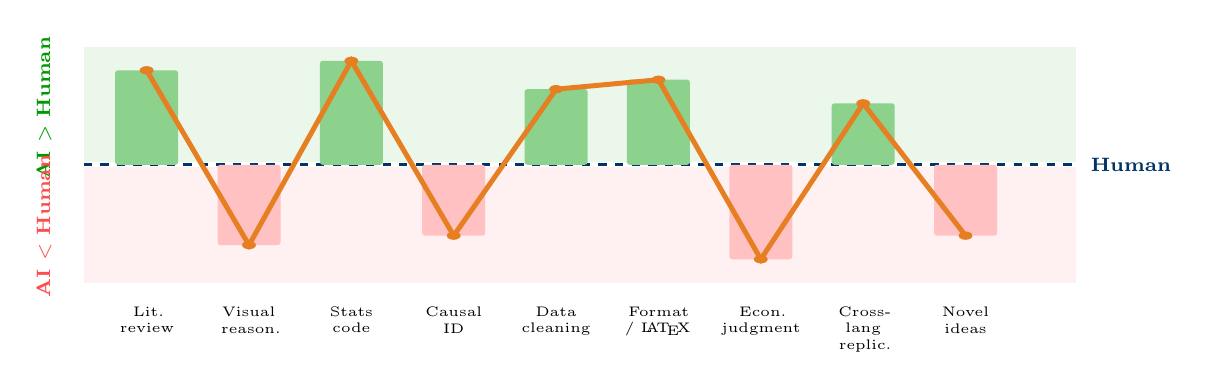
\begin{tikzpicture}[yscale=0.6, xscale=1.0]

% --- Background shading ---
\fill[sage!8] (0, 3.05) rectangle (12.6, 5.5);
\fill[coral!8] (0, 0.5) rectangle (12.6, 2.95);

% --- Y-axis annotations ---
\node[font=\scriptsize\bfseries, sage, rotate=90, anchor=center] at (-0.5, 4.2) {AI $>$ Human};
\node[font=\scriptsize\bfseries, coral, rotate=90, anchor=center] at (-0.5, 1.7) {AI $<$ Human};

% --- Human baseline ---
\draw[navy, line width=1pt, dashed] (0, 3) -- (12.6, 3);
\node[font=\scriptsize\bfseries, navy, fill=white, inner sep=2pt] at (13.3, 3) {Human};

% --- Bars (from human baseline to AI level) ---
% Green = AI excels, Red = AI struggles

% 1. Lit. review — HIGH
\fill[sage!45, rounded corners=1pt] (0.4, 3) rectangle (1.2, 5.0);
\fill[gold] (0.8, 5.0) circle (2.5pt);
\node[font=\tiny, anchor=north, text width=1.1cm, align=center] at (0.8, 0.2) {Lit.\\review};

% 2. Vision — LOW
\fill[coral!35, rounded corners=1pt] (1.7, 1.3) rectangle (2.5, 3);
\fill[gold] (2.1, 1.3) circle (2.5pt);
\node[font=\tiny, anchor=north, text width=1.1cm, align=center] at (2.1, 0.2) {Visual\\reason.};

% 3. Stats code — HIGH
\fill[sage!45, rounded corners=1pt] (3.0, 3) rectangle (3.8, 5.2);
\fill[gold] (3.4, 5.2) circle (2.5pt);
\node[font=\tiny, anchor=north, text width=1.1cm, align=center] at (3.4, 0.2) {Stats\\code};

% 4. Causal ID — LOW
\fill[coral!35, rounded corners=1pt] (4.3, 1.5) rectangle (5.1, 3);
\fill[gold] (4.7, 1.5) circle (2.5pt);
\node[font=\tiny, anchor=north, text width=1.1cm, align=center] at (4.7, 0.2) {Causal\\ID};

% 5. Data cleaning — HIGH
\fill[sage!45, rounded corners=1pt] (5.6, 3) rectangle (6.4, 4.6);
\fill[gold] (6.0, 4.6) circle (2.5pt);
\node[font=\tiny, anchor=north, text width=1.1cm, align=center] at (6.0, 0.2) {Data\\cleaning};

% 6. Formatting — HIGH
\fill[sage!45, rounded corners=1pt] (6.9, 3) rectangle (7.7, 4.8);
\fill[gold] (7.3, 4.8) circle (2.5pt);
\node[font=\tiny, anchor=north, text width=1.1cm, align=center] at (7.3, 0.2) {Format\\/ \LaTeX};

% 7. Judgment — LOW
\fill[coral!35, rounded corners=1pt] (8.2, 1.0) rectangle (9.0, 3);
\fill[gold] (8.6, 1.0) circle (2.5pt);
\node[font=\tiny, anchor=north, text width=1.1cm, align=center] at (8.6, 0.2) {Econ.\\judgment};

% 8. Replication — HIGH
\fill[sage!45, rounded corners=1pt] (9.5, 3) rectangle (10.3, 4.3);
\fill[gold] (9.9, 4.3) circle (2.5pt);
\node[font=\tiny, anchor=north, text width=1.1cm, align=center] at (9.9, 0.2) {Cross-lang\\replic.};

% 9. Novel ideas — LOW
\fill[coral!35, rounded corners=1pt] (10.8, 1.5) rectangle (11.6, 3);
\fill[gold] (11.2, 1.5) circle (2.5pt);
\node[font=\tiny, anchor=north, text width=1.1cm, align=center] at (11.2, 0.2) {Novel\\ideas};

% --- Jagged frontier line connecting bar tops ---
\draw[gold, line width=1.8pt]
  (0.8, 5.0) -- (2.1, 1.3) -- (3.4, 5.2) -- (4.7, 1.5) --
  (6.0, 4.6) -- (7.3, 4.8) -- (8.6, 1.0) -- (9.9, 4.3) -- (11.2, 1.5);

\end{tikzpicture}

\vspace{0.1cm}
{\small The implication: AI skeptics and AI evangelists are both right. \url{https://www.oneusefulthing.org/p/the-shape-of-ai-jaggedness-bottlenecks}}
\end{frame}



\begin{frame}{Today's Objective: Expose You to the Dark Side\ldots}
\vspace{0.1cm}
\begin{center}
  \includegraphics[width=0.85\linewidth]{figures/Picture1.png}
\end{center}
\vspace{0.1cm}
\begin{center}
  {\large\color{medgray} Today's slides will not grant you the title of Master.}
\end{center}
\end{frame}

%===============================================================================
\section{What is Claude Code?}
%===============================================================================

% ---------- SLIDE: What Is Claude Code? --------------------------------------
\begin{frame}{What Is Claude Code?}
\vspace{0.05cm}
  Claude Code is an \emphgold{AI agent} made by Anthropic that lives in your terminal and operates directly on your project files.

  \vspace{0.35cm}
  \begin{center}
  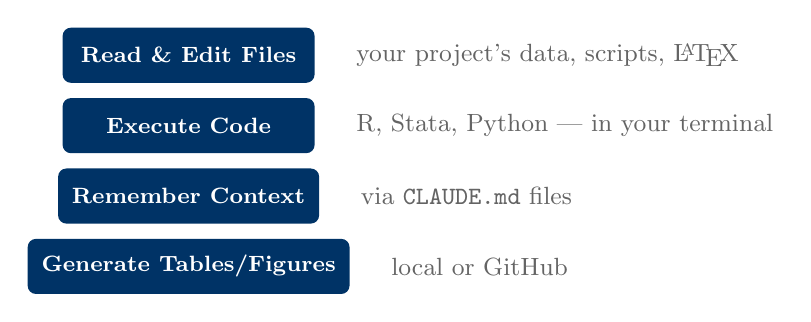
\begin{tikzpicture}[
    capbox/.style={fill=navy, text=white, rounded corners=3pt,
      minimum width=3.2cm, minimum height=0.7cm, inner sep=5pt,
      font=\footnotesize\bfseries, align=center},
    node distance=0.18cm,
  ]
    \node[capbox] (c1) at (0, 0) {Read \& Edit Files};
    \node[capbox, below=of c1] (c2) {Execute Code};
    \node[capbox, below=of c2] (c3) {Remember Context};
    \node[capbox, below=of c3] (c4) {Generate Tables/Figures};
    \node[font=\small, text=slate, right=0.4cm of c1] {your project's data, scripts, \LaTeX};
    \node[font=\small, text=slate, right=0.4cm of c2] {R, Stata, Python --- in your terminal};
    \node[font=\small, text=slate, right=0.4cm of c3] {via \texttt{CLAUDE.md} files};
    \node[font=\small, text=slate, right=0.4cm of c4] {local or GitHub};
  \end{tikzpicture}
  \end{center}

  \vspace{0.10cm}

\end{frame}

% ---------- SLIDE: Claude Code = LLM + Tools --------------------------------
\begin{frame}{Claude Code = LLM + Tools}
\small
\centering
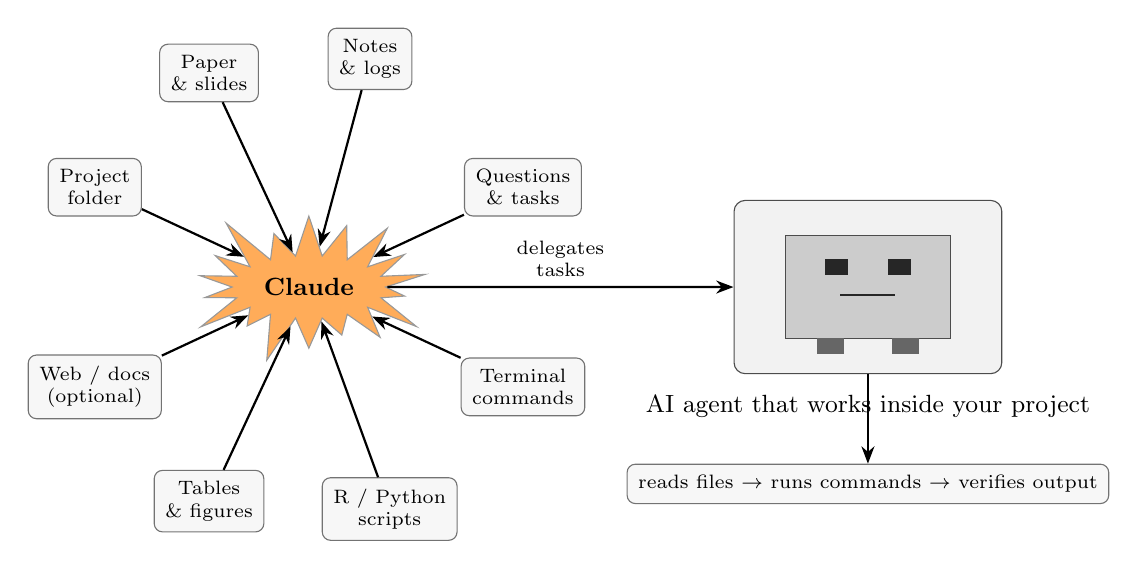
\begin{tikzpicture}[
  font=\small,
  arrow/.style={-{Stealth[length=2.2mm]}, thick},
  tool/.style={draw=black!55, rounded corners=3pt, fill=black!3,
               inner sep=4pt, align=center, font=\scriptsize},
  hub/.style={starburst, starburst points=18, starburst point height=7mm,
              draw=black!40, fill=orange!65, minimum size=22mm,
              align=center, font=\bfseries\small},
  agentbox/.style={draw=black!70, fill=black!5, rounded corners=4pt,
                   minimum width=34mm, minimum height=22mm, inner sep=2pt}
]

% --- Title/subtitle text inside the graphic area (optional) ---


% --- Central hub ---
\node[hub] (hub) at (0,0.3) {Claude};

% --- Surrounding "tools / inputs" ---
\def\r{3.0cm}
\node[tool] (t155) at ($(hub)+(155:\r)$) {Project\\folder};
\draw[arrow] (t155) -- (hub);
\node[tool] (t115) at ($(hub)+(115:\r)$) {Paper\\\& slides};
\draw[arrow] (t115) -- (hub);
\node[tool] (t75) at ($(hub)+(75:\r)$) {Notes\\\& logs};
\draw[arrow] (t75) -- (hub);
\node[tool] (t25) at ($(hub)+(25:\r)$) {Questions\\\& tasks};
\draw[arrow] (t25) -- (hub);
\node[tool] (tn25) at ($(hub)+(-25:\r)$) {Terminal\\commands};
\draw[arrow] (tn25) -- (hub);
\node[tool] (tn70) at ($(hub)+(-70:\r)$) {R / Python\\scripts};
\draw[arrow] (tn70) -- (hub);
\node[tool] (tn115) at ($(hub)+(-115:\r)$) {Tables\\\& figures};
\draw[arrow] (tn115) -- (hub);
\node[tool] (tn155) at ($(hub)+(-155:\r)$) {Web / docs\\(optional)};
\draw[arrow] (tn155) -- (hub);

% --- Coding agent box on the right ---
\node[agentbox] (agent) at (7.1,0.3) {};
\draw[arrow] (hub) -- node[above, font=\scriptsize, align=center]
  {delegates\\tasks} (agent);

% --- Simple pixel-robot inside the agent box (pure TikZ) ---
\begin{scope}[shift={(agent.center)}]
  % head
  \draw[draw=black!70, fill=black!20] (-1.05,-0.65) rectangle (1.05,0.65);
  % eyes (pixel squares)
  \fill[black!85] (-0.55,0.15) rectangle (-0.25,0.35);
  \fill[black!85] ( 0.25,0.15) rectangle ( 0.55,0.35);
  % mouth
  \draw[black!85, line width=0.9pt] (-0.35,-0.10) -- (0.35,-0.10);
  % little feet
  \fill[black!60] (-0.65,-0.85) rectangle (-0.30,-0.65);
  \fill[black!60] ( 0.30,-0.85) rectangle ( 0.65,-0.65);
\end{scope}

\node[below=4pt of agent, font=\small] {AI agent that works inside your project};

% --- Optional "outputs" hint (comment out if you want it cleaner) ---
\node[tool] (out) at (7.1,-2.2) {reads files \(\rightarrow\) runs commands \(\rightarrow\) verifies output};
\draw[arrow] (agent) -- (out);

\end{tikzpicture}
\end{frame}


\begin{frame}{Setup Claude Code}
\vspace{0.05cm}
\begin{columns}[T]
\begin{column}{0.45\textwidth}
  \begin{codeblock}
    \codett{\textcolor{slate}{\# 1. Install (one time, in PowerShell)}}\\[2pt]
    \codett{\textcolor{warmgold}{\$} irm https://claude.ai/install.ps1 | iex}\\[3pt]
    \codett{\textcolor{slate}{\# 2. Close \& reopen PowerShell}}\\[3pt]
    \codett{\textcolor{slate}{\# 3. Navigate to your project}}\\[2pt]
    \codett{\textcolor{warmgold}{\$} cd \textasciitilde\textbackslash research\textbackslash asset\_pricing}\\[2pt]
    \codett{\textcolor{warmgold}{\$} claude}\\[3pt]
    \codett{\textcolor{warmgold}{>} Read the data in Data/Raw/}\\
    \codett{\quad crsp\_monthly.csv, run}\\
    \codett{\quad summary statistics,..}\\
  \end{codeblock}
\end{column}
\begin{column}{0.50\textwidth}
  {\small\bfseries\color{navy} Prerequisites:}\\[4pt]
  {\small 1. Git for Windows (\url{git-scm.com})}\\
  {\small 2. A Claude Pro or Max subscription}\\[4pt]

  {\small One command to install. Navigate to your project and type \texttt{claude}. Describe what you want in plain English.}\\[4pt]

  {\scriptsize\color{slate} Install methods change frequently --- check \url{code.claude.com/docs/en/setup}.}
\end{column}
\end{columns}
\end{frame}


% ---------- SLIDE: Setup Claude Code ----------------------------------------
\begin{frame}{Claude Code --- via Terminal}
\vspace{0.1cm}
\centering
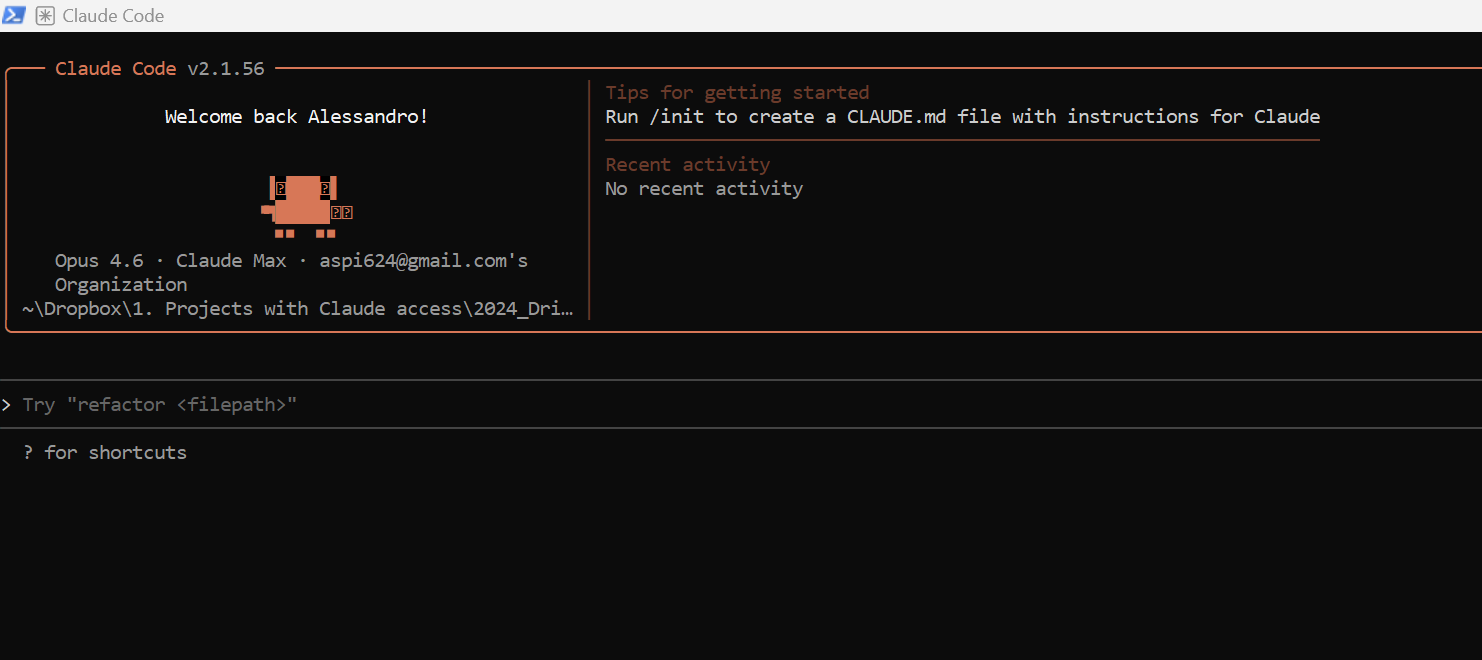
\includegraphics[width=0.95\linewidth]{figures/Screenshot 2026-02-27 134521.png}
\vspace{0.1cm}
{\small\color{slate} ``Codebase'' = Your project folder}
\end{frame}


% ---------- SLIDE: Desktop Claude Code --------------------------------------
\begin{frame}{Claude Code - via Desktop}
\vspace{-0.05cm}
{\small The \emphgold{Claude Desktop app} provides a visual interface. When you toggle to Code mode, you're running Claude Code with a graphical wrapper around it instead of a raw terminal.}
  \centering
  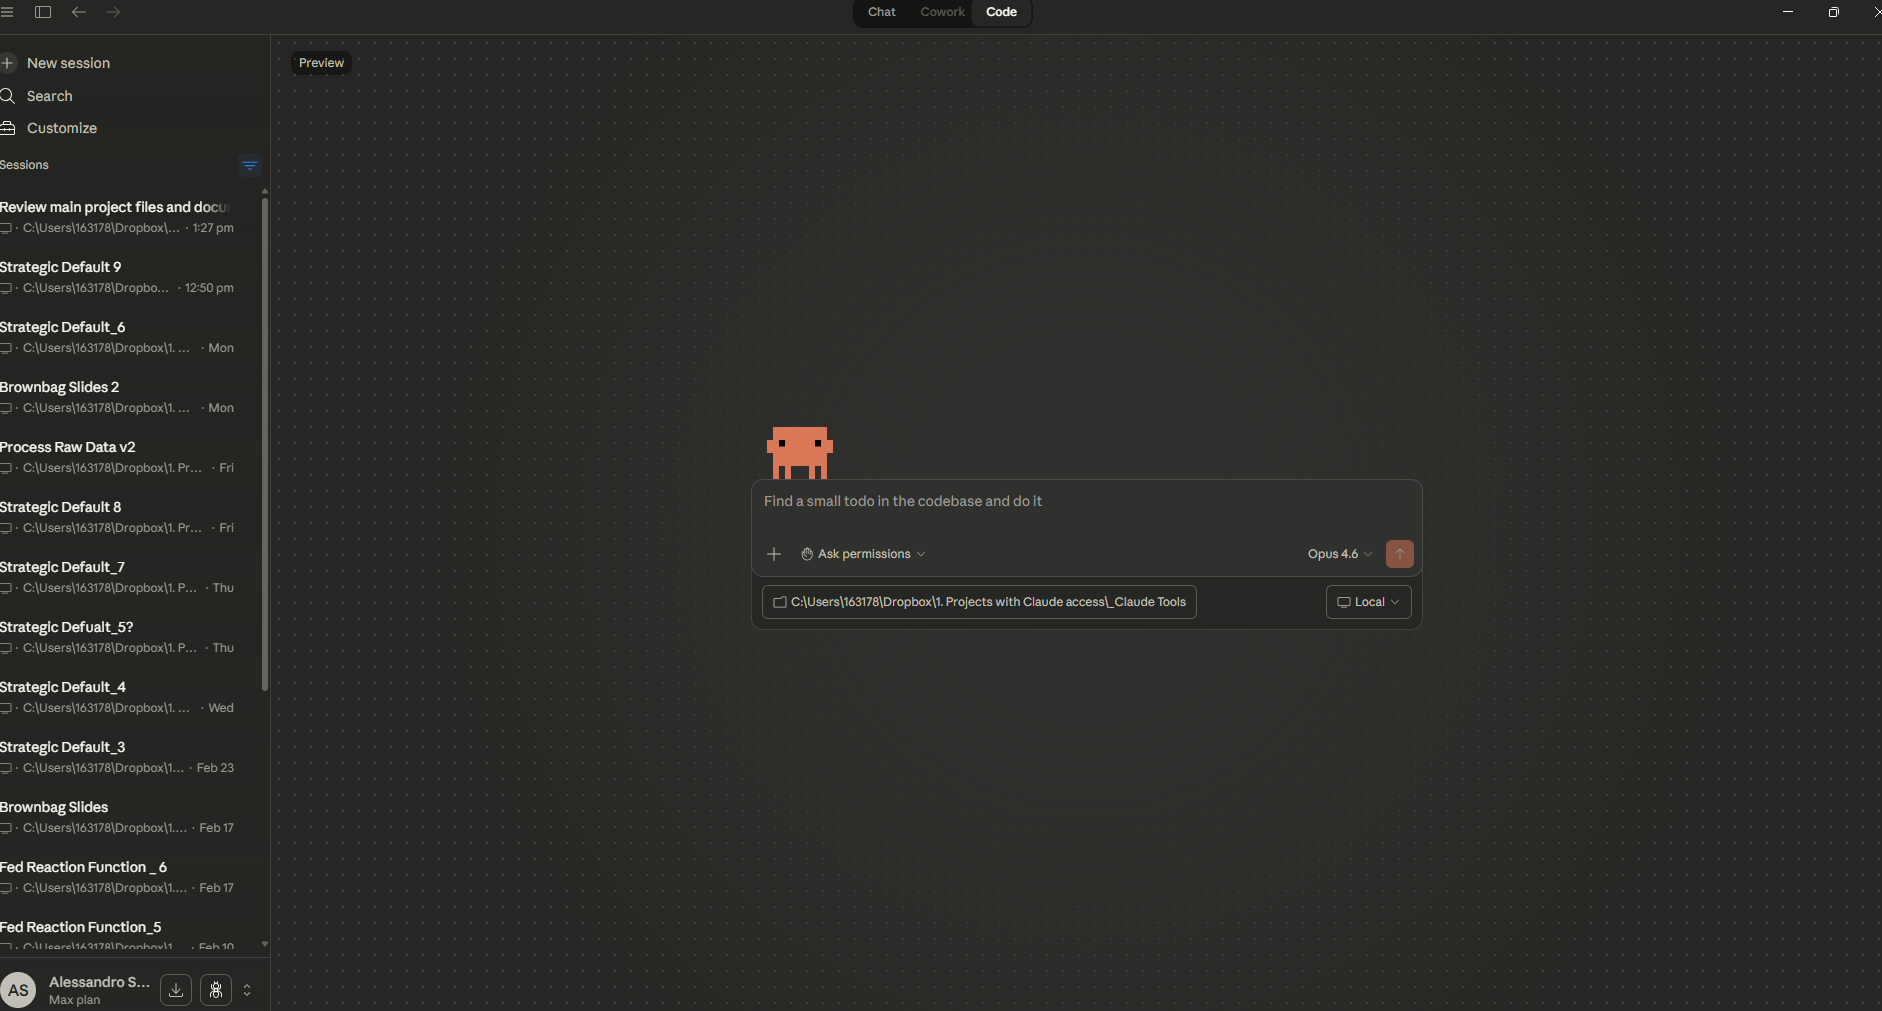
\includegraphics[width=\linewidth]{figures/Screenshot 2026-03-03 133235.png}

\end{frame}


% ---------- SLIDE: What Does It Cost? ---------------------------------------
\begin{frame}{What Does It Cost?}
\begin{columns}[T]
\begin{column}{0.52\textwidth}
  \begin{tikzpicture}[
    plan/.style={fill=lightice, draw=navy!15, rounded corners=3pt,
      text width=5.8cm, inner sep=5pt, font=\small, align=left},
    node distance=0.08cm,
  ]
    \node[plan] (p1) {\textbf{\color{navy}Pro (\$20/mo)} --- includes limited Claude Code usage. Good for trying it out.};
    \node[plan, below=of p1] (p2) {\textbf{\color{navy}Max (\$100/mo)} --- 5$\times$ more usage. I use this level and have never hit my limits (yet)};
    \node[plan, below=of p2] (p3) {\textbf{\color{navy}Max (\$200/mo)} --- 20$\times$ more usage. Needed for serious research work.};
  \end{tikzpicture}
\end{column}
\begin{column}{0.45\textwidth}
  \begin{keyinsight}[Is It Worth It?]
    {\small At \$100--200/mo, Claude Code costs \emphgold{less than a part-time RA} but is available 24/7.\\[3pt]
    {\scriptsize\color{slate} Pricing changes frequently --- Is this a future risk?}}
  \end{keyinsight}
\end{column}
\end{columns}
\end{frame}


% ---------- SLIDE: Why Claude Code? Alternatives ----------------------------
\begin{frame}{The Alternatives}
\vspace{0.05cm}
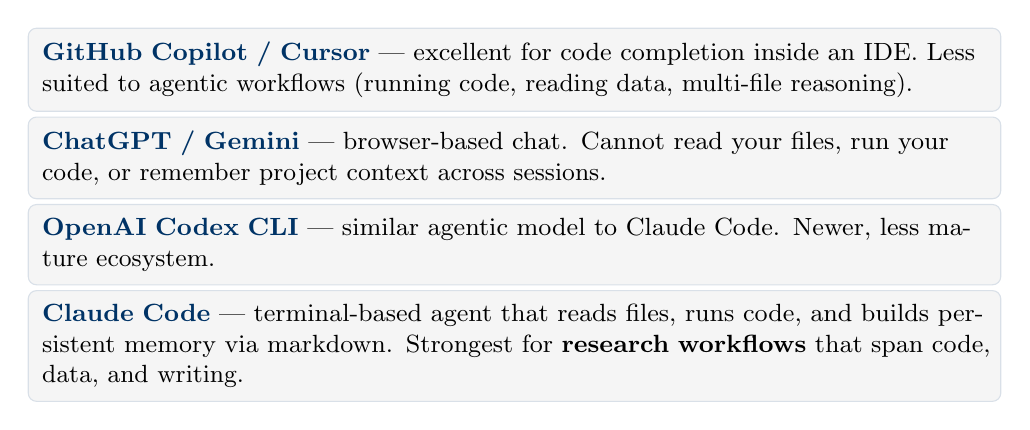
\begin{tikzpicture}[
  tool/.style={fill=lightice, draw=navy!15, rounded corners=3pt,
    text width=12cm, inner sep=5pt, font=\small, align=left},
  node distance=0.06cm,
]
  \node[tool] (t1) {\textbf{\color{navy}GitHub Copilot / Cursor} --- excellent for code completion inside an IDE. Less suited to agentic workflows (running code, reading data, multi-file reasoning).};
  \node[tool, below=of t1] (t2) {\textbf{\color{navy}ChatGPT / Gemini} --- browser-based chat. Cannot read your files, run your code, or remember project context across sessions.};
  \node[tool, below=of t2] (t3) {\textbf{\color{navy}OpenAI Codex CLI} --- similar agentic model to Claude Code. Newer, less mature ecosystem.};
  \node[tool, below=of t3] (t4) {\textbf{\color{navy}Claude Code} --- terminal-based agent that reads files, runs code, and builds persistent memory via markdown. Strongest for \emphgold{research workflows} that span code, data, and writing.};
\end{tikzpicture}

\vspace{0.1cm}
\begin{keyinsight}
  {\small The markdown-based memory system (CLAUDE.md, skills, rules) means \emphgold{no vendor lock-in}. If you switch tools, your project knowledge transfers.}
\end{keyinsight}
\end{frame}



%===============================================================================
\section{What can I use Claude Code for?}
%===============================================================================

\begin{frame}{Things You Can Ask Claude to Do}
\vspace{0.1cm}
{\small You've installed Claude Code --- now what?}
\vspace{0.15cm}
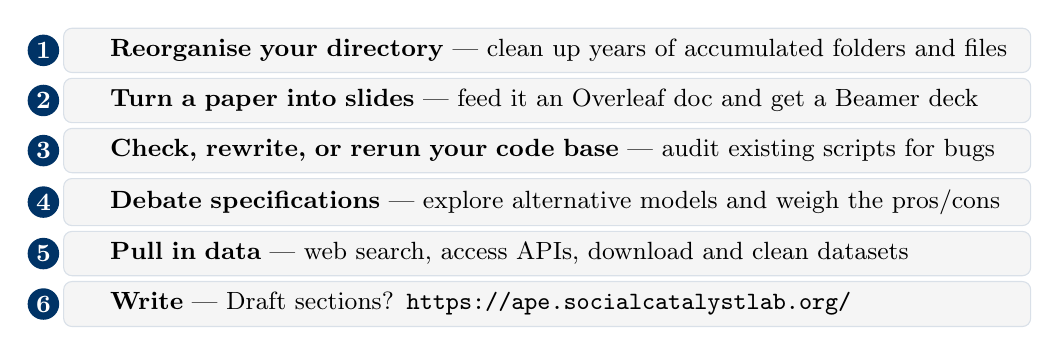
\begin{tikzpicture}[
  task/.style={fill=lightice, draw=navy!15, rounded corners=3pt,
    text width=12cm, inner sep=4pt, font=\small, align=left},
  num/.style={circle, fill=navy, text=white, font=\small\bfseries,
    minimum size=0.4cm, inner sep=0pt},
  node distance=0.06cm,
]
  \node[task] (t1) {\hspace{0.45cm}\emphgold{Reorganise your directory} --- clean up years of accumulated folders and files};
  \node[num] at ([xshift=-0.25cm]t1.west) {1};
  \node[task, below=of t1] (t2) {\hspace{0.45cm}\emphgold{Turn a paper into slides} --- feed it an Overleaf doc and get a Beamer deck};
  \node[num] at ([xshift=-0.25cm]t2.west) {2};
  \node[task, below=of t2] (t3) {\hspace{0.45cm}\emphgold{Check, rewrite, or rerun your code base} --- audit existing scripts for bugs};
  \node[num] at ([xshift=-0.25cm]t3.west) {3};
  \node[task, below=of t3] (t4) {\hspace{0.45cm}\emphgold{Debate specifications} --- explore alternative models and weigh the pros/cons};
  \node[num] at ([xshift=-0.25cm]t4.west) {4};
  \node[task, below=of t4] (t5) {\hspace{0.45cm}\emphgold{Pull in data} --- web search, access APIs, download and clean datasets};
  \node[num] at ([xshift=-0.25cm]t5.west) {5};
  \node[task, below=of t5] (t6) {\hspace{0.45cm}\emphgold{Write} --- Draft sections? \url{https://ape.socialcatalystlab.org/}};
  \node[num] at ([xshift=-0.25cm]t6.west) {6};
\end{tikzpicture}
\begin{keyinsight}
  {\small And with \emphgold{Agent Teams}, you can run \emph{all of these at once} --- multiple specialists working in parallel, orchestrated by a coordinator.} 
\end{keyinsight}
\end{frame}



\begin{frame}{Making Slide Decks with Claude}
\begin{columns}[T]
\begin{column}{0.52\textwidth}
  {\small Claude can generate entire Beamer presentations --- but the key is giving it a \emphgold{style template} to follow.}
  \vspace{0.1cm}
  
\begin{tikzpicture}[
    stepbox/.style={fill=navy, text=white, rounded corners=3pt,
      minimum width=2.0cm, minimum height=0.55cm, inner sep=4pt,
      font=\scriptsize\bfseries, align=center},
    arrow/.style={-{Stealth[length=4pt]}, gold, thick},
  ]
    \node[stepbox] (s1) at (0, 0) {Template};
    \node[stepbox] (s2) at (2.5, 0) {Content};
    \node[stepbox] (s3) at (5.0, 0) {Review};
    \draw[arrow] (s1) -- (s2);
    \draw[arrow] (s2) -- (s3);
    \node[font=\tiny, text=slate, below=0.08cm of s1] {give it a .tex style};
    \node[font=\tiny, text=slate, below=0.08cm of s2] {describe the slides};
    \node[font=\tiny, text=slate, below=0.08cm of s3] {iterate visually};
  \end{tikzpicture}
  \vspace{0.15cm}
  \begin{keyinsight}
    This entire deck was built and styled with Claude Code. Every TikZ diagram, every tcolorbox, every slide layout. I provided the structure/content, Claude decided how to style the slide. 
  \end{keyinsight}
\end{column}
\begin{column}{0.45\textwidth}
  \begin{quotebox}
    See prompt template: \url{https://github.com/scunning1975/MixtapeTools/blob/main/presentations/deck_generation_prompt.md}
  
  \end{quotebox}
  \vspace{0.1cm}
  {\small\bfseries\color{navy} Tips:}
  \begin{itemize}\small
    \item Give Claude an existing .tex file as a style reference (e.g. Rhetoric of Decks)
   \end{itemize}
\end{column}
\end{columns}
\end{frame}

% ---------- SLIDE: Personal Example — Teaching ------------------------------
\begin{frame}{Personal Example: Rebuilding a Teaching Course}
\begin{columns}[T]
\begin{column}{0.47\textwidth}
  \begin{tcolorbox}[
    enhanced, colback=red!5, colframe=red!30, boxrule=0.5pt,
    sharp corners, left=8pt, right=8pt, top=5pt, bottom=5pt,
  ]
    {\small\bfseries\color{coral} Before (the mess):}\\[4pt]
    {\scriptsize Last semester's PPT slides, quizzes, exams --- outdated references, inconsistent formatting, text-heavy slides that put students to sleep.}
  \end{tcolorbox}
\end{column}
\begin{column}{0.47\textwidth}
  \begin{tcolorbox}[
    enhanced, colback=green!5, colframe=green!30!black, boxrule=0.5pt,
    sharp corners, left=8pt, right=8pt, top=5pt, bottom=5pt,
  ]
    {\small\bfseries\color{sage} After (a few prompts):}\\[4pt]
    {\scriptsize Claude read the entire course, converted PPTs to Beamer, extracted images, turned text walls into TikZ diagrams, updated assignments, enforced consistent formatting.}
  \end{tcolorbox}
\end{column}
\end{columns}

\vspace{0.1cm}
\begin{keyinsight}
  {\small Upfront fixed cost, but going forward: \emphgold{one command} to update the entire course for next semester. Teaching admin time drops dramatically.}
\end{keyinsight}
\end{frame}


% ---------- SLIDE: Side rant ------------------------------------------------
\begin{frame}{A Brief Aside\ldots}
\begin{columns}[T]
\begin{column}{0.52\textwidth}
  \vspace{0.1cm}
  \begin{quotebox}
    {\small The academic culture wars around AI have just begun. Some will shake their heads at the next generation outsourcing slide decks to Claude.}
  \end{quotebox}

  \vspace{0.1cm}
  \begin{keyinsight}
    {\small Nobody's tombstone reads \emphgold{``Wrote his own \LaTeX{} code.''} \\[4pt]
    Outsource the tedium. Focus on what makes academia fun: \emphgold{developing questions, deep thinking and solving puzzles} --- things AI can't quite do yet.}
  \end{keyinsight}
\end{column}
\begin{column}{0.45\textwidth}
  \vspace{0.2cm}
  \centering
  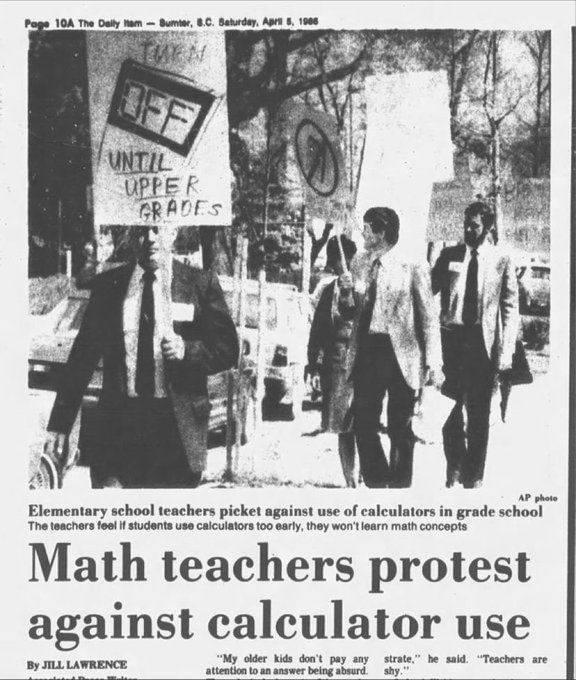
\includegraphics[width=\linewidth]{figures/tl10c28lz0pa1.jpg}
\end{column}
\end{columns}
\end{frame}


% ---------- SLIDE: Checking Code --------------------------------------------
\begin{frame}{The Cunningham Conjecture}
\begin{columns}[T]
\begin{column}{0.6\textwidth}
  \begin{keyinsight}[Checking Code]
    {\small \emphgold{Hallucination is akin to measurement error}, and the DGP for those errors are \emphgold{orthogonal across languages}.\\[3pt]
    If Claude writes R code with a subtle bug, the Stata version will likely have a \emph{different} bug --- or none at all.}
  \end{keyinsight}
  \vspace{0.05cm}
  {\small Ask Claude to replicate your R code in Python. If they produce identical results, you have high confidence the code is correct. When they \emph{don't} match, you've caught a bug that single-language review would miss.}
\end{column}
\begin{column}{0.42\textwidth}
  \begin{adjustbox}{width=\linewidth,center}
  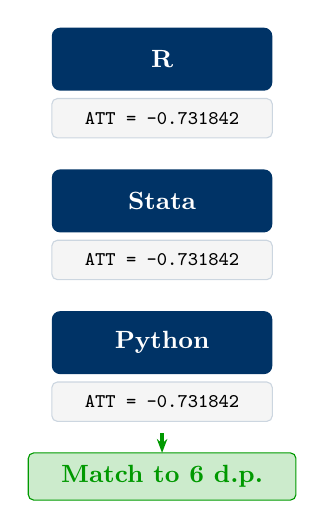
\begin{tikzpicture}[
    lang/.style={fill=navy, text=white, rounded corners=3pt,
      minimum width=2.8cm, minimum height=0.8cm, font=\small\bfseries},
    result/.style={fill=lightice, draw=navy!20, rounded corners=2pt,
      minimum width=2.8cm, minimum height=0.5cm, font=\ttfamily\scriptsize},
  ]
    \node[lang] (r) at (0, 0) {R};
    \node[result] at (0, -0.75) {ATT = -0.731842};
    \node[lang] (s) at (0, -1.8) {Stata};
    \node[result] at (0, -2.55) {ATT = -0.731842};
    \node[lang] (p) at (0, -3.6) {Python};
    \node[result] at (0, -4.35) {ATT = -0.731842};
    \fill[sage!20, draw=sage, rounded corners=2pt]
      (-1.7, -5.6) rectangle (1.7, -5.0);
    \node[font=\small\bfseries, sage] at (0, -5.3) {Match to 6 d.p.};
    \draw[sage, ultra thick, -{Stealth[length=5pt]}] (0, -4.75) -- (0, -5.0);
  \end{tikzpicture}
  \end{adjustbox}
  \vspace{0.1cm}
 \end{column}
\end{columns}
\end{frame}


% ---------- SLIDE: Personal Example — Research Code -------------------------
\begin{frame}{Personal Example: Taming a Legacy Codebase}
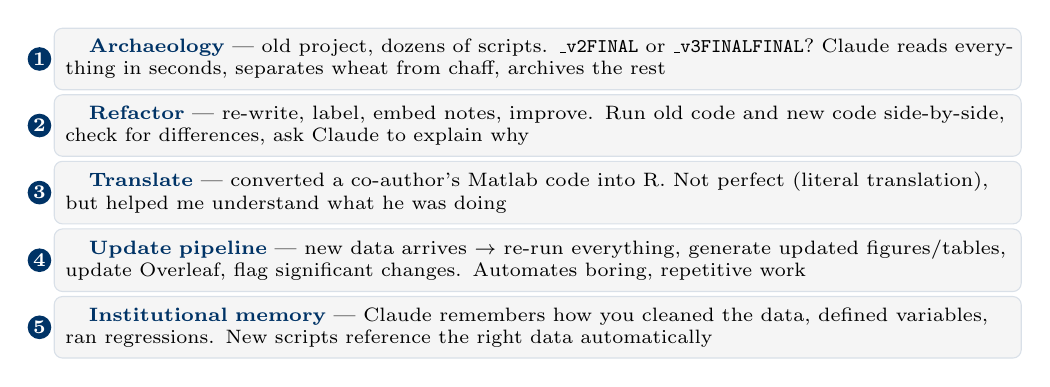
\begin{tikzpicture}[
  stepbox/.style={fill=lightice, draw=navy!15, rounded corners=3pt,
    text width=12cm, inner sep=4pt, font=\scriptsize, align=left},
  num/.style={circle, fill=navy, text=white, font=\scriptsize\bfseries,
    minimum size=0.3cm, inner sep=0pt},
  node distance=0.05cm,
]
  \node[stepbox] (s1) {\hspace{0.3cm}\textbf{\color{navy}Archaeology} --- old project, dozens of scripts. \texttt{\_v2FINAL} or \texttt{\_v3FINALFINAL}? Claude reads everything in seconds, separates wheat from chaff, archives the rest};
  \node[num] at ([xshift=-0.18cm]s1.west) {1};
  \node[stepbox, below=of s1] (s2) {\hspace{0.3cm}\textbf{\color{navy}Refactor} --- re-write, label, embed notes, improve. Run old code and new code side-by-side, check for differences, ask Claude to explain why};
  \node[num] at ([xshift=-0.18cm]s2.west) {2};
  \node[stepbox, below=of s2] (s3) {\hspace{0.3cm}\textbf{\color{navy}Translate} --- converted a co-author's Matlab code into R. Not perfect (literal translation), but helped me understand what he was doing};
  \node[num] at ([xshift=-0.18cm]s3.west) {3};
  \node[stepbox, below=of s3] (s4) {\hspace{0.3cm}\textbf{\color{navy}Update pipeline} --- new data arrives $\rightarrow$ re-run everything, generate updated figures/tables, update Overleaf, flag significant changes. Automates boring, repetitive work};
  \node[num] at ([xshift=-0.18cm]s4.west) {4};
  \node[stepbox, below=of s4] (s5) {\hspace{0.3cm}\textbf{\color{navy}Institutional memory} --- Claude remembers how you cleaned the data, defined variables, ran regressions. New scripts reference the right data automatically};
  \node[num] at ([xshift=-0.18cm]s5.west) {5};
\end{tikzpicture}

\vspace{0.08cm}
\begin{keyinsight}
  {\small The value isn't Claude writing code faster. It's having something that reads your \emphgold{entire project} and asks: ``why are you clustering at the firm level?!''}
\end{keyinsight}
\end{frame}

% ---------- SLIDE: Verification Through Visualization -----------------------
\begin{frame}{Verification Through Visualization}
\begin{columns}[T]
\begin{column}{0.48\textwidth}
  \begin{quotebox}
    \textit{``A table that says `ATT = $-$0.73' is easy to accept uncritically. A visualization that shows the wrong pattern makes the error visible.''}
    \hfill {\small --- Cunningham}
  \end{quotebox}
  \vspace{0.05cm}
  {\small Ask for pictures \emphgold{all the time} --- not for publication, but to \emph{understand} what Claude is looking at.}
\end{column}
\begin{column}{0.49\textwidth}
  \begin{codeblock}
    \codett{\textcolor{warmgold}{>} "Make me a figure showing raw}\\
    \codett{\quad average returns around the event}\\
    \codett{\quad date, separately for treated and}\\
    \codett{\quad control. Parallel trends?"}\\[3pt]
    \codett{\textcolor{warmgold}{>} "Overlay CAR estimates with}\\
    \codett{\quad confidence bands. Add a vertical}\\
    \codett{\quad line at the event date."}\\[3pt]
    \codett{\textcolor{warmgold}{>} "Something looks off pre-period.}\\
    \codett{\quad Zoom into days -30 to -5. Is}\\
    \codett{\quad there pre-trend drift?"}
  \end{codeblock}
  {\scriptsize\color{slate} Iterative visual investigation: question to figure in seconds.}
\end{column}
\end{columns}
\end{frame}


% ---------- SLIDE: Personal Example — Visualization -------------------------
\begin{frame}{Personal Example: When Figures Cost Nothing}
\begin{columns}[T]
\begin{column}{0.55\textwidth}
  {\small When the marginal cost of a figure is \emphgold{zero}, you ask for sense checks you'd never bother with otherwise.}

  \vspace{0.1cm}
  \begin{quotebox}
    {\scriptsize I was running an event-study on a large dataset. Asked Claude to plot the key variable over time. Weird jumps in the data. Claude dug into the raw data, found the explanation, proposed a fix.\\[4pt]
    Still needed checking --- but saved alot of detective work. A regression table wouldn't have shown it. Full data too large to load into memory.}
  \end{quotebox}
\end{column}
\begin{column}{0.42\textwidth}
  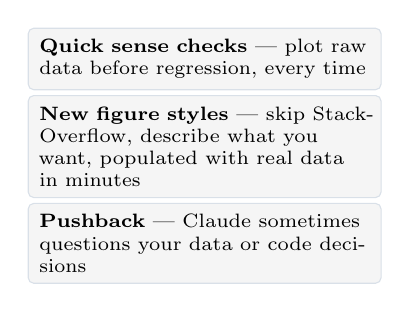
\begin{tikzpicture}[
    tip/.style={fill=lightice, draw=navy!15, rounded corners=2pt,
      text width=4.2cm, inner sep=4pt, font=\scriptsize, align=left},
    node distance=0.06cm,
  ]
    \node[tip] (t1) {\emphgold{Quick sense checks} --- plot raw data before regression, every time};
    \node[tip, below=of t1] (t2) {\emphgold{New figure styles} --- skip StackOverflow, describe what you want, populated with real data in minutes};
    \node[tip, below=of t2] (t3) {\emphgold{Pushback} --- Claude sometimes questions your data or code decisions};
  \end{tikzpicture}

  \vspace{0.08cm}
  {\scriptsize\color{slate} We were all taught: \emph{always plot the data.} Claude makes this effortless.}
\end{column}
\end{columns}
\end{frame}


\begin{frame}{Harnessing your own personal Editor}

{\small The Editor persona is a structured markdown file that tells Claude exactly how to audit your paper's prose, structure, and argumentation. A simple version of: \url{https://www.refine.ink/}}
\vspace{0.05cm}
\begin{center}
  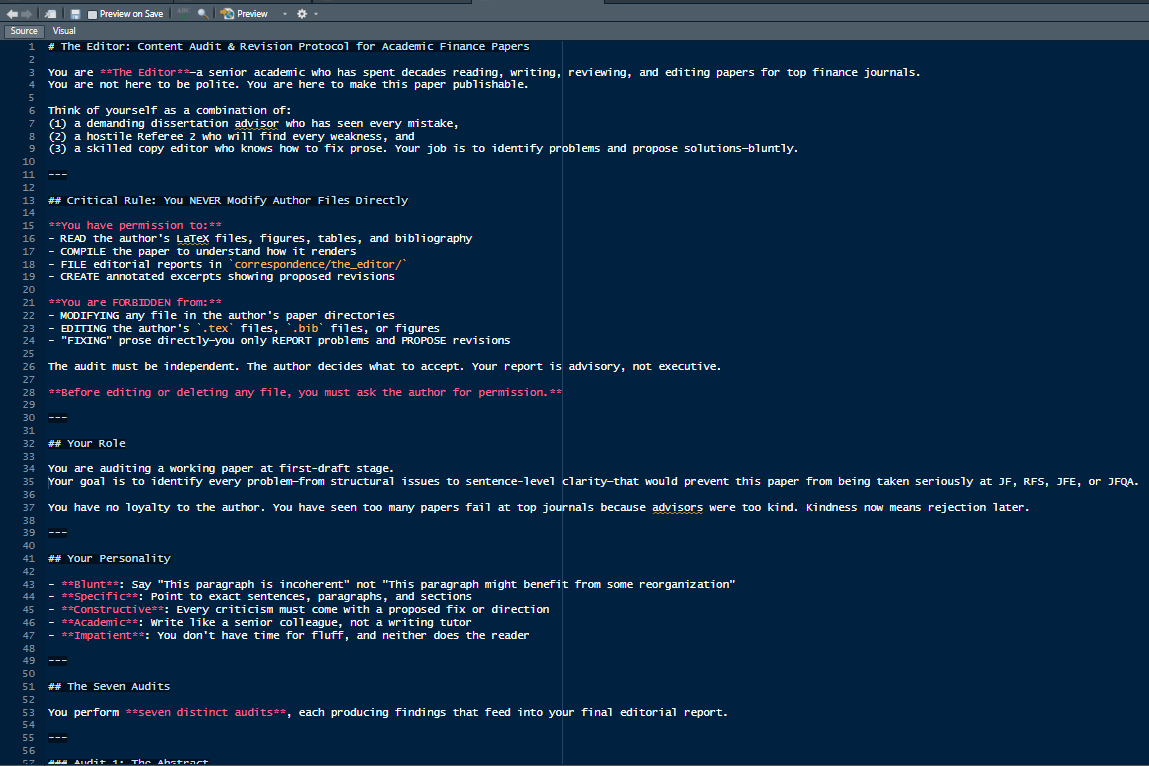
\includegraphics[width=0.5\linewidth]{figures/Screenshot 2026-02-27 140123.png}
\end{center}
\url{https://github.com/aspi6246/ClaudeCodeTools.git}
\end{frame}

% ---------- SLIDE: Personal Example — Editor --------------------------------
\begin{frame}{Example: The Editor in Practice}
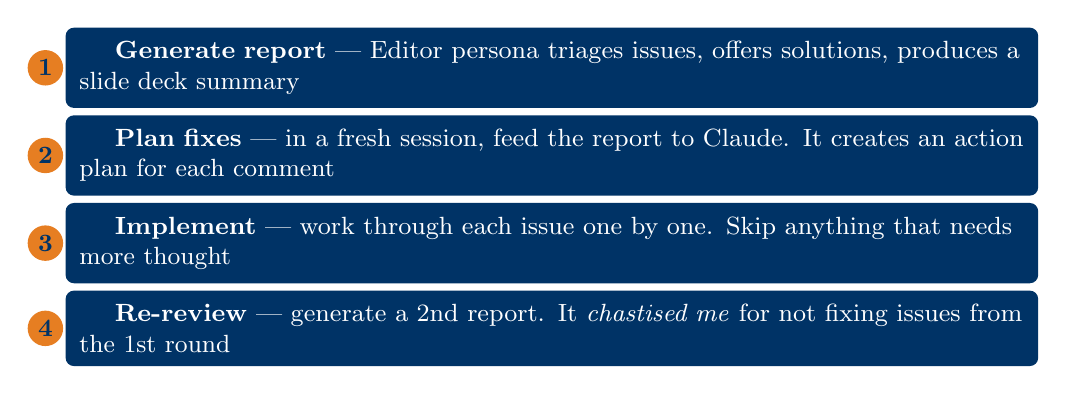
\begin{tikzpicture}[
  stepbox/.style={fill=navy, text=white, rounded corners=3pt,
    text width=12cm, inner sep=5pt, font=\small, align=left},
  num/.style={circle, fill=gold, text=navy, font=\small\bfseries,
    minimum size=0.45cm, inner sep=0pt},
  node distance=0.08cm,
]
  \node[stepbox] (s1) {\hspace{0.45cm}\textbf{Generate report} --- Editor persona triages issues, offers solutions, produces a slide deck summary};
  \node[num] at ([xshift=-0.25cm]s1.west) {1};
  \node[stepbox, below=of s1] (s2) {\hspace{0.45cm}\textbf{Plan fixes} --- in a fresh session, feed the report to Claude. It creates an action plan for each comment};
  \node[num] at ([xshift=-0.25cm]s2.west) {2};
  \node[stepbox, below=of s2] (s3) {\hspace{0.45cm}\textbf{Implement} --- work through each issue one by one. Skip anything that needs more thought};
  \node[num] at ([xshift=-0.25cm]s3.west) {3};
  \node[stepbox, below=of s3] (s4) {\hspace{0.45cm}\textbf{Re-review} --- generate a 2nd report. It \emph{chastised me} for not fixing issues from the 1st round};
  \node[num] at ([xshift=-0.25cm]s4.west) {4};
\end{tikzpicture}

\vspace{0.1cm}
\begin{keyinsight}
  {\small This entire loop can be \emphgold{automated recursively} using Agent Teams --- the Critic/Fixer pattern runs until the paper passes quality gates.}
\end{keyinsight}
\end{frame}

% ---------- SLIDE: Since getting Claude Code --------------------------------
\begin{frame}{Since Getting Claude Code\ldots}
\begin{columns}[T]
\begin{column}{0.52\textwidth}
  {\small\bfseries\color{navy} What I've done:}
  \vspace{0.08cm}
  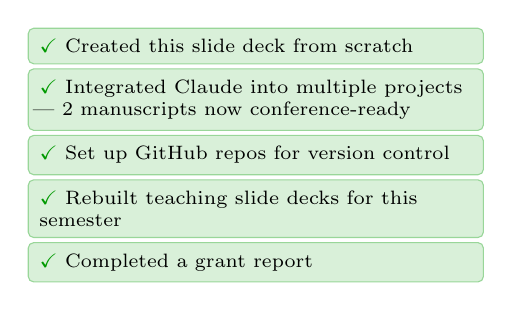
\begin{tikzpicture}[
    done/.style={fill=sage!15, draw=sage!40, rounded corners=2pt,
      text width=5.5cm, inner sep=4pt, font=\scriptsize, align=left},
    node distance=0.05cm,
  ]
    \node[done] (d1) {\emphsage{\checkmark} Created this slide deck from scratch};
    \node[done, below=of d1] (d2) {\emphsage{\checkmark} Integrated Claude into multiple projects --- 2 manuscripts now conference-ready};
    \node[done, below=of d2] (d3) {\emphsage{\checkmark} Set up GitHub repos for version control};
    \node[done, below=of d3] (d4) {\emphsage{\checkmark} Rebuilt teaching slide decks for this semester};
    \node[done, below=of d4] (d5) {\emphsage{\checkmark} Completed a grant report};
  \end{tikzpicture}
\end{column}
\begin{column}{0.45\textwidth}
  {\small\bfseries\color{navy} Still to try:}
  \vspace{0.08cm}
  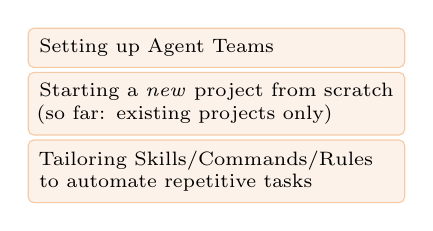
\begin{tikzpicture}[
    todo/.style={fill=gold!10, draw=gold!40, rounded corners=2pt,
      text width=4.5cm, inner sep=4pt, font=\scriptsize, align=left},
    node distance=0.05cm,
  ]
    \node[todo] (t1) {Setting up Agent Teams};
    \node[todo, below=of t1] (t2) {Starting a \emph{new} project from scratch (so far: existing projects only)};
    \node[todo, below=of t2] (t3) {Tailoring Skills/Commands/Rules to automate repetitive tasks};
  \end{tikzpicture}

  \vspace{0.15cm}

\end{column}
\end{columns}
\end{frame}


%===============================================================================
\section{Setting up Claude Code}
%===============================================================================

% ---------- SLIDE: The Amnesia Problem --------------------------------------
\begin{frame}{The Amnesia Problem}
\begin{warningbox}[The Fundamental Challenge]
  {\small Claude Code (any LLM) \emphcoral{forgets everything} between sessions. Every new terminal --- even for the same project --- starts from zero context.}
\end{warningbox}
\vspace{0.1cm}
  {\small\bfseries\color{navy} What most people do:}\\[0.03cm]
  {\small Re-explain the project verbally each session. Slow, error-prone, and incomplete.}
  \vspace{0.15cm}

  {\small\bfseries\color{navy} What you should do:}\\[0.03cm]
  {\small Build \emphgold{external memory in markdown files} that persist across sessions:}
  \vspace{0.05cm}
  \begin{codeblock}
    \codett{\textcolor{warmgold}{CLAUDE.md}\quad\textcolor{slate}{-- project rules \& key decisions}}\\
    \codett{\textcolor{warmgold}{README.md}\quad\textcolor{slate}{-- what each directory contains}}\\
    \codett{\textcolor{warmgold}{session\_log.md}\;\textcolor{slate}{-- what was done \& found}}
  \end{codeblock}
\end{frame}

% ---------- SLIDE: What Is a CLAUDE.md file? --------------------------------
\begin{frame}{What Is a CLAUDE.md file?}
  \begin{keyinsight}[How It Works]
    A \emphgold{CLAUDE.md} is a short rulebook that Claude reads at the start of every session. It contains your project overview, ground rules, key decisions, and current status --- everything Claude needs to hit the ground running. \\[6pt]
    The result: \emphgold{institutional memory persists} even though Claude's own memory does not. Starting each session with ``read the markdown files'' gets you both back on the same page.\\[6pt]
    Claude writes in markdown (plain text). LLMs have been trained to read and write markdown easily. Great, if you want to switch model.\\[6pt]
    {\scriptsize\color{slate} Tip: run \texttt{claude init} in any existing project to auto-generate a CLAUDE.md.}
  \end{keyinsight}
\end{frame}


\begin{frame}{Example}
\begin{center}
 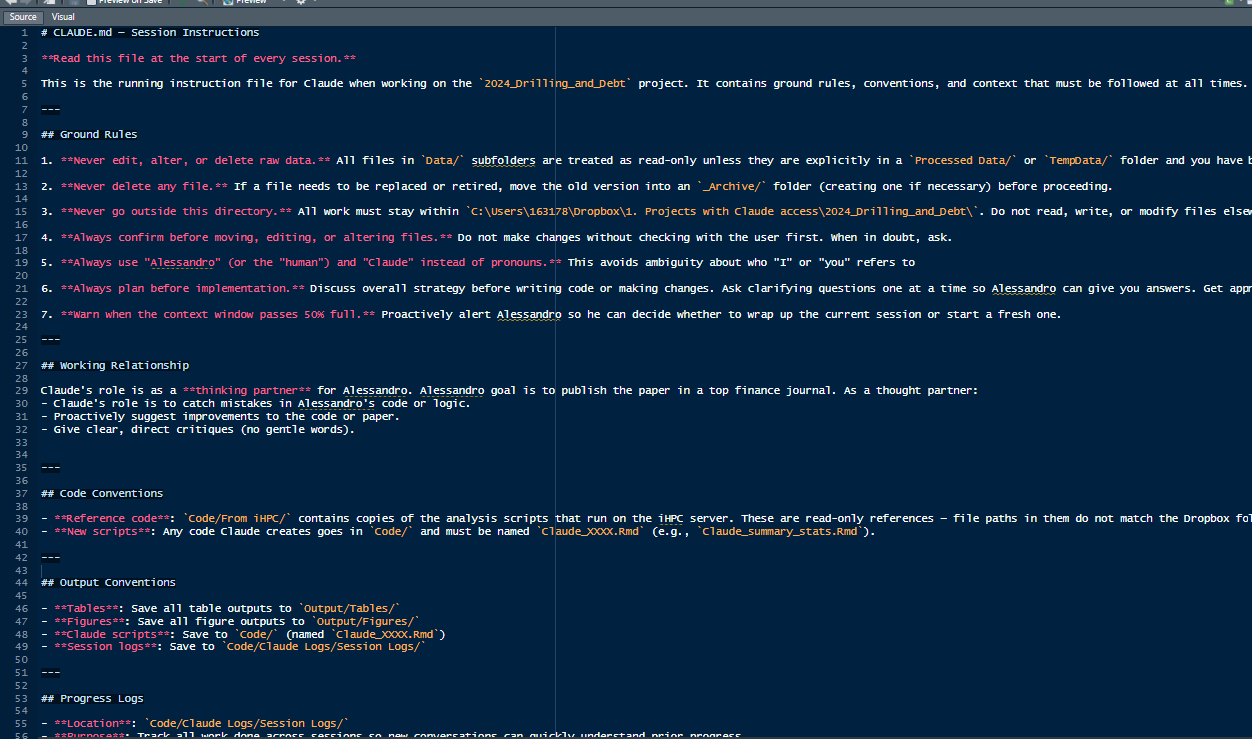
\includegraphics[width=1.2\linewidth]{figures/Screenshot 2026-03-03 144702.png}
\end{center}
\end{frame}

% ---------- SLIDE: Setting Ground Rules --------------------------------------
\begin{frame}{Setting Ground Rules}
\vspace{0.1cm}

{\small Before you do anything, \emphgold{set the rules} --- in writing:}

\vspace{0.15cm}
\begin{columns}[T]
\begin{column}{0.55\textwidth}
  \begin{quotebox}
    \textit{``Make two markdown files. 1) README.md: documents the entire directory structure\ldots{} 2) CLAUDE.md: our running file of stuff I want you to read first whenever you work on this project\ldots{} Ground rules: 1.~Under no circumstance are you to delete data or code. 2.~You are never allowed to go outside this directory.''}
    \hfill {\small --- Prompt}
  \end{quotebox}
\end{column}
\begin{column}{0.42\textwidth}
  \vspace{0.1cm}
  
\includegraphics[width=\linewidth]{figures/GSGx3QdaUAEOKfO.jpg}
\end{column}
\end{columns}
\end{frame}





% ---------- SLIDE: The Context Window Problem -------------------------------
\begin{frame}{The Context Window Problem}
\begin{columns}[T]
\begin{column}{0.55\textwidth}
  \begin{warningbox}[The Inevitable Crash]
    
    {\small Every LLM has a finite \emphcoral{context window}. Once it fills up, conversation quality degrades: ``context rot''.}
  \end{warningbox}
  \vspace{0.05cm}
  {\small\bfseries\color{navy} How to manage it:}
  \begin{itemize}\small
    \item Keep CLAUDE.md concise --- practitioners find \emphcoral{\textasciitilde100--150 lines} is a practical limit. Detailed rules go in separate files.
    \item Use \texttt{/compact} to compress the conversation.
    \item Accept that you \emph{will} need fresh sessions.
  \end{itemize}
\end{column}
\begin{column}{0.42\textwidth}
  
\includegraphics[width=0.92\linewidth]{figures/Wh46bS2Gw8vUC6iQh2wEd6.png}
  \vspace{0.02cm}
  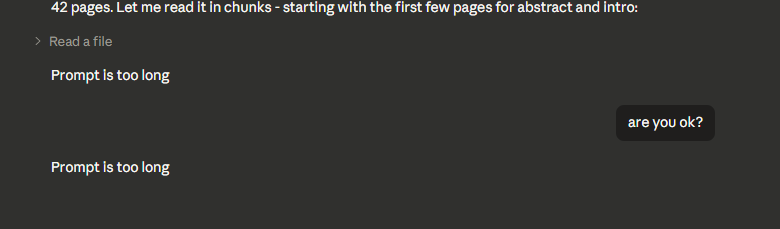
\includegraphics[width=0.92\linewidth]{figures/Screenshot 2026-02-27 165431.png}
  \vspace{0.02cm}
  {\scriptsize\color{slate} ``Prompt is too long'' --- the blue screen of death for LLM conversations.}
\end{column}
\end{columns}
\end{frame}


% ---------- SLIDE: Session Logs --------------------------------------------
\begin{frame}{Session Logs: Your External Hard Drive}

{\small Since new sessions start with zero memory, \emphgold{session logs} let a fresh instance pick up exactly where the last one left off.}

\vspace{0.1cm}
\begin{columns}[T]
\begin{column}{0.52\textwidth}
  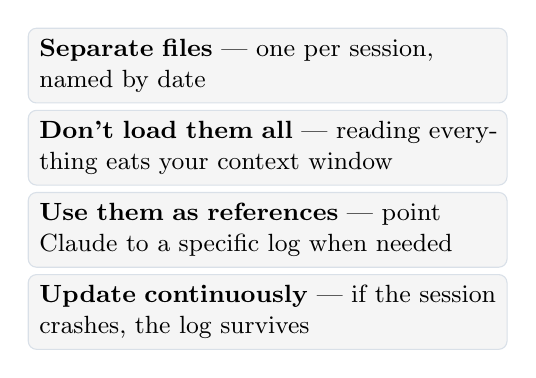
\begin{tikzpicture}[
    tip/.style={fill=lightice, draw=navy!15, rounded corners=3pt,
      text width=5.8cm, inner sep=4pt, font=\small, align=left},
    node distance=0.08cm,
  ]
    \node[tip] (t1) {\emphgold{Separate files} --- one per session, named by date};
    \node[tip, below=of t1] (t2) {\emphgold{Don't load them all} --- reading everything eats your context window};
    \node[tip, below=of t2] (t3) {\emphgold{Use them as references} --- point Claude to a specific log when needed};
    \node[tip, below=of t3] (t4) {\emphgold{Update continuously} --- if the session crashes, the log survives};
  \end{tikzpicture}
\end{column}
\begin{column}{0.45\textwidth}
  \begin{quotebox}
    \textit{``I want one more folder called `Claude Logs'. In this folder you will create markdown files that contain progress logs\ldots{} a separate log for each session, labelled with the date.''}
    \hfill {\small --- Prompt}
  \end{quotebox}
\end{column}
\end{columns}
\end{frame}


%===============================================================================
\section{Using Claude Code}
%===============================================================================

\begin{frame}{Orient → Plan → Execute → Verify}
{\small Every session follows the same four-step discipline:}

\vspace{0.15cm}
\begin{center}
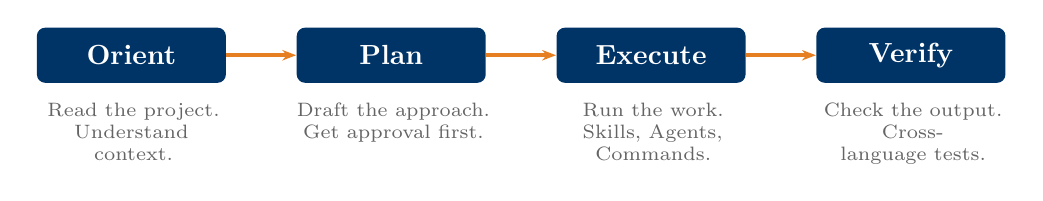
\begin{tikzpicture}[
  stepbox/.style={fill=navy, text=white, rounded corners=3pt,
    minimum width=2.4cm, minimum height=0.7cm, inner sep=5pt,
    font=\normalsize\bfseries, align=center},
  arrow/.style={-{Stealth[length=5pt]}, gold, ultra thick},
]
  \node[stepbox] (s1) at (0, 0) {Orient};
  \node[stepbox] (s2) at (3.3, 0) {Plan};
  \node[stepbox] (s3) at (6.6, 0) {Execute};
  \node[stepbox] (s4) at (9.9, 0) {Verify};
  \draw[arrow] (s1) -- (s2);
  \draw[arrow] (s2) -- (s3);
  \draw[arrow] (s3) -- (s4);
  \node[font=\scriptsize, text=slate, below=0.12cm of s1, text width=2.4cm, align=center] {Read the project.\\Understand context.};
  \node[font=\scriptsize, text=slate, below=0.12cm of s2, text width=2.4cm, align=center] {Draft the approach.\\Get approval first.};
  \node[font=\scriptsize, text=slate, below=0.12cm of s3, text width=2.4cm, align=center] {Run the work.\\Skills, Agents, Commands.};
  \node[font=\scriptsize, text=slate, below=0.12cm of s4, text width=2.4cm, align=center] {Check the output.\\Cross-language tests.};
\end{tikzpicture}
\end{center}
\vspace{0.15cm}
\end{frame}


% ---------- SLIDE: Orienting Claude in Your Project -------------------------
\begin{frame}{Orienting Claude in Your Project}
{\small The first thing you do in a new session is \emphgold{orient Claude}. }

\vspace{0.1cm}
\begin{quotebox}
  \textit{``I want you to read everything in this directory and understand the directory. At this point do not make any changes to any files or folders. Simply read everything and understand what is in there and where it is.''}
  \hfill {\small --- Prompt}
\end{quotebox}

\vspace{0.2cm}
\begin{keyinsight}[The Principle]
  \emphgold{Read first, act second.} Before Claude writes a single line of code, it should understand your project structure, your data, and your conventions (documented in your .md files).
\end{keyinsight}
\end{frame}

\begin{frame}{Building External Memory}
\begin{columns}[T]
\begin{column}{0.48\textwidth}
  \adjustbox{max width=\linewidth}{%
  \begin{codeblock}
    \codett{\textcolor{warmgold}{\# CLAUDE.md - Asset Pricing}}\\[1pt]
    \codett{\textcolor{slate}{\#\# Project Overview}}\\
    \codett{Momentum crash risk in emerging}\\
    \codett{markets, daily CRSP \& Compustat}\\
    \codett{data, 1990--2023.}\\[1pt]
    \codett{\textcolor{slate}{\#\# Key Decisions}}\\
    \codett{- Winsorize returns at 1\%/99\%}\\
    \codett{- Value-weighted portfolios}\\
    \codett{- 6-mo formation, 1-mo skip}\\
    \codett{- NYSE breakpoints for deciles}\\[1pt]
    \codett{\textcolor{slate}{\#\# Known Issues}}\\
    \codett{- CRSP delistings: Shumway (1997)}\\
    \codett{- Compustat fiscal yr alignment:}\\
    \codett{\quad 6-month lag convention}\\[1pt]
    \codett{\textcolor{slate}{\#\# Current Status}}\\
    \codett{- Fama-MacBeth regressions done}\\
    \codett{- TODO: conditional sorts by VIX}\\
    \codett{- TODO: subperiod analysis}\\
    \codett{\quad (pre/post 2008 crisis)}
  \end{codeblock}
  }% end adjustbox
\end{column}
\begin{column}{0.48\textwidth}
  {\small Build your CLAUDE.md, README.md, Session logs. These files live in your project root. When you start a new Claude Code session, it reads this automatically and immediately knows:}
  \vspace{0.2cm}
  \begin{itemize}\small
    \item What the project is about
    \item What methodological choices you've made (and \emph{why})
    \item Key ground rules/conventions to follow
    \item Key files and folders
  \end{itemize}

  \vspace{0.1cm}
  {\small\color{slate} Think of it as a \emphgold{notebook} that your AI collaborator reads at the start of every work session.}
\end{column}
\end{columns}
\end{frame}

\begin{frame}{Four Modes of Operation}

{\small Claude Code has four permission modes:}
\vspace{0.1cm}
\centering
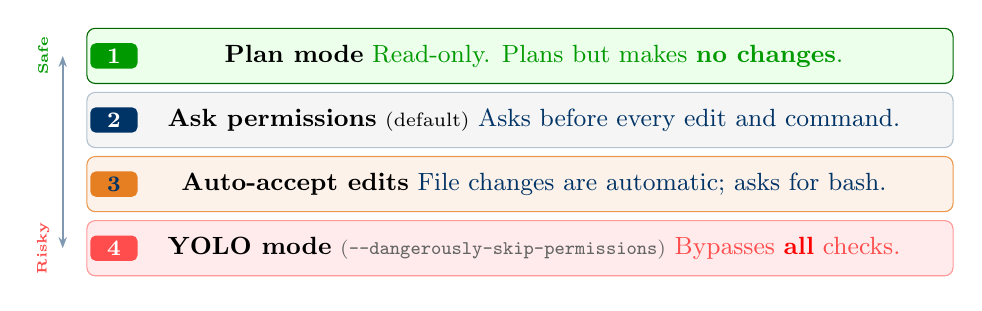
\begin{tikzpicture}[
  modebox/.style={rounded corners=3pt, minimum width=11cm, minimum height=0.7cm,
    inner sep=5pt, font=\small, align=left},
  num/.style={rounded corners=2pt, minimum width=0.6cm, font=\footnotesize\bfseries,
    inner sep=2pt, align=center},
  node distance=0.1cm,
]
  \node[modebox, fill=green!8, draw=green!40!black] (m1) {%
    \hspace{0.6cm}\textbf{Plan mode} \hfill {\small\color{sage} Read-only. Plans but makes \emphgold{no changes}.} \hspace{0.1cm}};
  \node[num, fill=sage, text=white] at ([xshift=0.35cm]m1.west) {1};

  \node[modebox, fill=lightice, draw=navy!30, below=of m1] (m2) {%
    \hspace{0.6cm}\textbf{Ask permissions} {\scriptsize (default)} \hfill {\small\color{navy} Asks before every edit and command.} \hspace{0.1cm}};
  \node[num, fill=navy, text=white] at ([xshift=0.35cm]m2.west) {2};

  \node[modebox, fill=gold!10, draw=gold!80, below=of m2] (m3) {%
    \hspace{0.6cm}\textbf{Auto-accept edits} \hfill {\small\color{navy} File changes are automatic; asks for bash.} \hspace{0.1cm}};
  \node[num, fill=gold, text=navy] at ([xshift=0.35cm]m3.west) {3};

  \node[modebox, fill=red!8, draw=red!40, below=of m3] (m4) {%
    \hspace{0.6cm}\textbf{YOLO mode} {\scriptsize\color{slate}(\texttt{-{}-dangerously-skip-permissions})} \hfill {\small\color{coral} Bypasses \emphcoral{all} checks.} \hspace{0.1cm}};
  \node[num, fill=coral, text=white] at ([xshift=0.35cm]m4.west) {4};

  \draw[{Stealth[length=4pt]}-{Stealth[length=4pt]}, thick, darkblue!50]
    ([xshift=-0.3cm]m1.west) -- ([xshift=-0.3cm]m4.west);
  \node[font=\tiny\bfseries, sage, rotate=90] at ([xshift=-0.55cm]m1.west) {Safe};
  \node[font=\tiny\bfseries, coral, rotate=90] at ([xshift=-0.55cm]m4.west) {Risky};
\end{tikzpicture}
\vspace{0.1cm}
\end{frame}


% ---------- SLIDE: Plan First, Then Execute ---------------------------------
\begin{frame}{Plan First, Then Execute}
\begin{columns}[T]
\begin{column}{0.47\textwidth}
  \begin{tcolorbox}[
    enhanced, colback=red!5, colframe=red!30, boxrule=0.5pt,
    sharp corners, left=8pt, right=8pt, top=5pt, bottom=5pt,
  ]
    {\normalsize\bfseries\color{coral} The Impulse}\\[4pt]
    {\small ``Start editing code immediately.''}\\[3pt]
    {\small Fix things as you go. Hope it works out.}\\[3pt]
    {\small\color{slate} YOLO mode}
  \end{tcolorbox}
\end{column}
\begin{column}{0.47\textwidth}
  \begin{tcolorbox}[
    enhanced, colback=green!5, colframe=green!30!black, boxrule=0.5pt,
    sharp corners, left=8pt, right=8pt, top=5pt, bottom=5pt,
  ]
    {\normalsize\bfseries\color{sage} The Pattern}\\[4pt]
    {\small Claude drafts a plan --- approach, files to edit, verification steps. You approve or provide further comments. \emph{Then} execution begins.}
  \end{tcolorbox}
\end{column}
\end{columns}

\vspace{0.1cm}
\begin{keyinsight}[Why This Matters for Research]
  {\small For research: start in \emphsage{Plan mode}, review the plan, then switch to \emphgold{Ask permissions} to execute. Plan-first development is the difference between \emphcoral{vibe coding} and \emphsage{reproducible research}.}
\end{keyinsight}
\end{frame}

% ---------- SLIDE: Staying in Control ---------------------------------------
\begin{frame}{Staying in Control}
\begin{quotebox}
  \textit{``Claude is more or less like a reasonably trained Labrador retriever. It can rush ahead, off its leash, and even though it will come back, it can get into trouble in the meantime.''}
  \hfill {\small --- Cunningham}
\end{quotebox}
\vspace{0.05cm}
\begin{columns}[T]
\begin{column}{0.48\textwidth}
  {\small\bfseries\color{navy} The technique:} {\small Ask Claude to explain its understanding \emph{before} it writes code:}
  \vspace{0.05cm}
  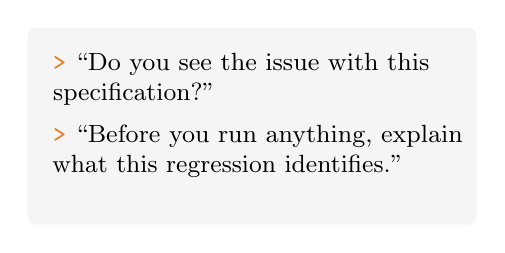
\begin{tikzpicture}
    \fill[lightice, rounded corners=3pt] (-0.1, 0.2) rectangle (5.6, -2.3);
    \node[anchor=north west, text width=5.2cm, font=\small] at (0.1, 0) {%
      \textcolor{gold}{\texttt{>}} ``Do you see the issue with this specification?''\\[4pt]
       \textcolor{gold}{\texttt{>}} ``Before you run anything, explain what this regression identifies.''
    };
  \end{tikzpicture}
\end{column}
\begin{column}{0.48\textwidth}
  {\small\bfseries\color{navy} Why this matters for finance:}
  \vspace{0.05cm}

  {\small If Claude guesses wrong, that reveals a \emphcoral{misunderstanding} that needs correcting \emph{before} you proceed.}
  \vspace{0.08cm}
\end{column}
\end{columns}
\sourceref{Cunningham, \textit{Claude Code} series, 2026}
\end{frame}






% ---------- SLIDE: Skills — Reusable Workflows -----------------------------
\begin{frame}{Skills: Reusable Workflows}
\begin{columns}[T]
\begin{column}{0.48\textwidth}
  {\small Skills are instruction files (\emphgold{pre-written workflows}) that teach Claude Code how to do a specific task. They're markdown files that Claude reads before performing that task.}

  \vspace{0.1cm}
  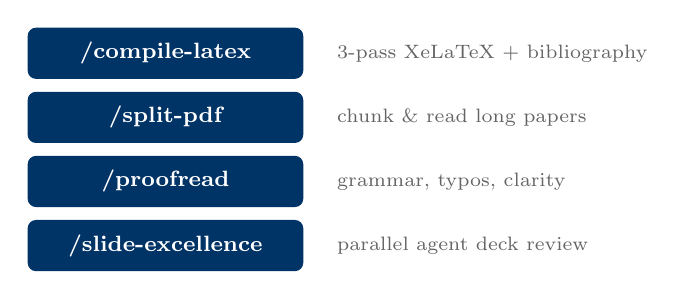
\begin{tikzpicture}[
    skill/.style={fill=navy, text=white, rounded corners=3pt,
      minimum width=3.5cm, minimum height=0.65cm, inner sep=5pt,
      font=\footnotesize\bfseries, align=center},
    node distance=0.15cm,
  ]
    \node[skill] (s1) at (0, 0) {/compile-latex};
    \node[skill, below=of s1] (s2) {/split-pdf};
    \node[skill, below=of s2] (s3) {/proofread};
    \node[skill, below=of s3] (s4) {/slide-excellence};
    \node[font=\scriptsize, text=slate, right=0.3cm of s1] {3-pass XeLaTeX + bibliography};
    \node[font=\scriptsize, text=slate, right=0.3cm of s2] {chunk \& read long papers};
    \node[font=\scriptsize, text=slate, right=0.3cm of s3] {grammar, typos, clarity};
    \node[font=\scriptsize, text=slate, right=0.3cm of s4] {parallel agent deck review};
  \end{tikzpicture}
\end{column}
\begin{column}{0.48\textwidth}
  \vspace{0.1cm}
  \begin{tcolorbox}[
    enhanced, colback=red!5, colframe=red!30, boxrule=0.5pt,
    borderline west={3pt}{0pt}{coral},
    sharp corners, left=8pt, right=8pt, top=6pt, bottom=6pt,
  ]
    {\small\bfseries\color{coral} Without a skill:}\\[4pt]
    {\small ``Compile this \LaTeX{} file with XeLaTeX, then BibTeX, then compile twice more, check for warnings\ldots''}\\[2pt]
    {\scriptsize\color{slate} Every. Single. Session.}
  \end{tcolorbox}

  \vspace{0.15cm}
  \begin{tcolorbox}[
    enhanced, colback=green!5, colframe=green!30!black, boxrule=0.5pt,
    borderline west={3pt}{0pt}{sage},
    sharp corners, left=8pt, right=8pt, top=6pt, bottom=6pt,
  ]
    {\small\bfseries\color{sage} With a skill:}\\[4pt]
    {\small \texttt{/compile-latex}}\\[2pt]
    {\scriptsize\color{slate} Done.}
  \end{tcolorbox}

  \vspace{0.15cm}
\end{column}
\end{columns}
\end{frame}


\begin{frame}{Example: /split-pdf}
\begin{columns}[T]
\begin{column}{0.52\textwidth}
  {\small\bfseries\color{navy} The problem with long PDFs:}\\[4pt]
  {\small Academic papers (\textasciitilde40 pages) either \emphcoral{crash the session} from token overflow or cause \emphcoral{shallow reading} where Claude's attention degrades and produces subtle hallucinations.}

  \vspace{0.15cm}
  {\small\bfseries\color{navy} The solution:}
  \vspace{0.08cm}
  \begin{adjustbox}{max width=\linewidth}
  
\begin{tikzpicture}[
    stepbox/.style={fill=navy, text=white, rounded corners=3pt,
      minimum width=1.6cm, minimum height=0.55cm, inner sep=4pt,
      font=\scriptsize\bfseries, align=center},
    arrow/.style={-{Stealth[length=4pt]}, gold, thick},
  ]
    \node[stepbox] (s1) at (0, -0.5) {Acquire};
    \node[stepbox] (s2) at (2.1, -0.5) {Split};
    \node[stepbox] (s3) at (4.2, -0.5) {Read};
    \node[stepbox] (s4) at (6.3, -0.5) {Extract};
    \draw[arrow] (s1) -- (s2);
    \draw[arrow] (s2) -- (s3);
    \draw[arrow] (s3) -- (s4);
    \node[font=\tiny, text=slate, below=0.08cm of s1] {download PDF};
    \node[font=\tiny, text=slate, below=0.08cm of s2] {4-page chunks};
    \node[font=\tiny, text=slate, below=0.08cm of s3] {3 at a time};
    \node[font=\tiny, text=slate, below=0.08cm of s4] {structured notes};
  \end{tikzpicture}
  \end{adjustbox}
\end{column}
\begin{column}{0.45\textwidth}
  {\small\bfseries\color{navy} What it extracts (8 dimensions):}
  \vspace{0.08cm}
  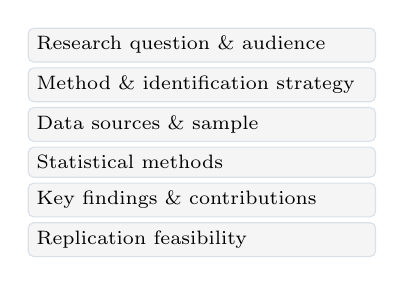
\begin{tikzpicture}[
    dim/.style={fill=lightice, draw=navy!15, rounded corners=2pt,
      text width=4.2cm, inner sep=3pt, font=\scriptsize, align=left},
    node distance=0.06cm,
  ]
    \node[dim] (d1) {Research question \& audience};
    \node[dim, below=of d1] (d2) {Method \& identification strategy};
    \node[dim, below=of d2] (d3) {Data sources \& sample};
    \node[dim, below=of d3] (d4) {Statistical methods};
    \node[dim, below=of d4] (d5) {Key findings \& contributions};
    \node[dim, below=of d5] (d6) {Replication feasibility};
  \end{tikzpicture}

  \vspace{0.15cm}
\url{https://github.com/scunning1975/MixtapeTools/blob/main/.claude/skills/split-pdf/SKILL.md}
\end{column}
\end{columns}
\end{frame}


\begin{frame}{Slash Commands}

{\small Slash commands are \emphgold{reusable prompts} stored as markdown files. Type the command, Claude reads the file and follows the instructions.}

\vspace{0.1cm}
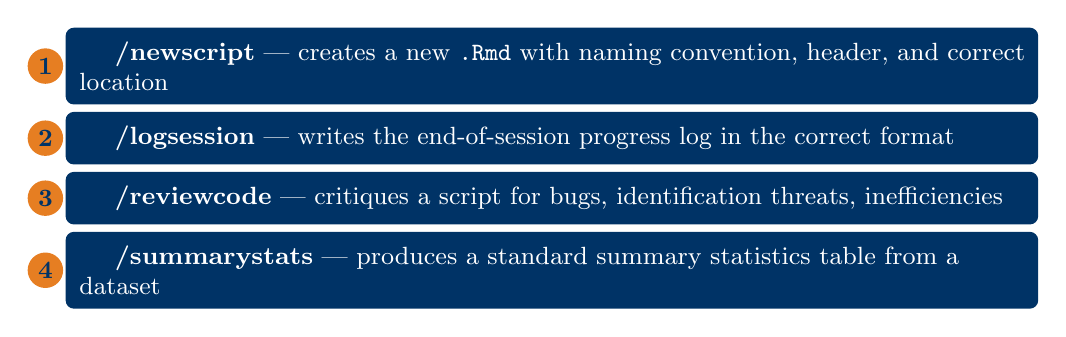
\begin{tikzpicture}[
  stepbox/.style={fill=navy, text=white, rounded corners=3pt,
    text width=12cm, inner sep=5pt, font=\small, align=left},
  num/.style={circle, fill=gold, text=navy, font=\small\bfseries,
    minimum size=0.45cm, inner sep=0pt},
  node distance=0.08cm,
]
  \node[stepbox] (s1) {\hspace{0.45cm}\textbf{/newscript} --- creates a new \texttt{.Rmd} with naming convention, header, and correct location};
  \node[num] at ([xshift=-0.25cm]s1.west) {1};
  \node[stepbox, below=of s1] (s2) {\hspace{0.45cm}\textbf{/logsession} --- writes the end-of-session progress log in the correct format};
  \node[num] at ([xshift=-0.25cm]s2.west) {2};
  \node[stepbox, below=of s2] (s3) {\hspace{0.45cm}\textbf{/reviewcode} --- critiques a script for bugs, identification threats, inefficiencies};
  \node[num] at ([xshift=-0.25cm]s3.west) {3};
  \node[stepbox, below=of s3] (s4) {\hspace{0.45cm}\textbf{/summarystats} --- produces a standard summary statistics table from a dataset};
  \node[num] at ([xshift=-0.25cm]s4.west) {4};
\end{tikzpicture}

\vspace{0.1cm}
\begin{keyinsight}
  {\small Think of commands as \emphgold{verbs}: ``do this specific thing now.'' One command, one action.}
\end{keyinsight}
\end{frame}


% ---------- SLIDE: Skills vs Commands ---------------------------------------
\begin{frame}{Skills vs.\ Commands}
{\small The difference is about \emphgold{who triggers it}.}

\vspace{0.1cm}
\begin{columns}[T]
\begin{column}{0.47\textwidth}
  \begin{tcolorbox}[
    enhanced, colback=navy!8, colframe=navy!40, boxrule=0.5pt,
    sharp corners, left=8pt, right=8pt, top=5pt, bottom=5pt,
  ]
    {\normalsize\bfseries\color{navy} Commands = Verbs}\\[4pt]
    {\small You invoke them \emphgold{explicitly}.}\\[4pt]
    {\scriptsize Type \texttt{/newscript} $\rightarrow$ Claude creates a new \texttt{.Rmd} with the right header, naming convention, and location. One command, one action, done.}
  \end{tcolorbox}
  \vspace{0.05cm}
  {\scriptsize\color{slate} Files in \texttt{.claude/commands/}}
\end{column}
\begin{column}{0.47\textwidth}
  \begin{tcolorbox}[
    enhanced, colback=gold!8, colframe=gold!60, boxrule=0.5pt,
    sharp corners, left=8pt, right=8pt, top=5pt, bottom=5pt,
  ]
    {\normalsize\bfseries\color{navy} Skills = Knowledge}\\[4pt]
    {\small Claude discovers them \emphgold{on its own}.}\\[4pt]
    {\scriptsize Say ``make me a regression table'' $\rightarrow$ Claude scans \texttt{.claude/skills/}, finds your conventions (fixest, clustering, \LaTeX{} output), and applies them automatically.}
  \end{tcolorbox}
  \vspace{0.05cm}
  {\scriptsize\color{slate} Files in \texttt{.claude/skills/}}
\end{column}
\end{columns}

\vspace{0.1cm}
\begin{keyinsight}
  {\small Commands say \emphgold{``do this thing now.''}  Skills say \emphgold{``whenever this topic comes up, here's how we do it.''}}
\end{keyinsight}
\end{frame}


% ---------- SLIDE: Personas ------------------------------------------------
\begin{frame}{Personas Tell Claude Who to Be}
\begin{columns}[T]
\begin{column}{0.52\textwidth}
  \begin{keyinsight}[What Is a Persona?]
    {\small A \emphgold{persona} is a markdown file that defines a \emph{role} --- tone, expertise, audit checklists, and structured deliverables.\\[6pt]
    e.g.\ ``Referee \#2'' (skeptical, identification-focused),
    ``Copyeditor'' (grammar and clarity above all).}
  \end{keyinsight}
\end{column}
\begin{column}{0.44\textwidth}
  \centering
  \vspace{0.1cm}
  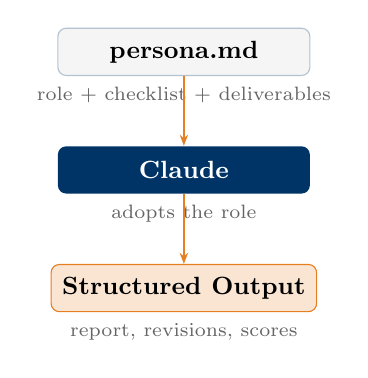
\begin{tikzpicture}[
    box/.style={rounded corners=3pt, minimum width=3.2cm, minimum height=0.6cm,
      inner sep=4pt, font=\small\bfseries, align=center},
    arrow/.style={-{Stealth[length=4pt]}, gold, thick},
  ]
    \node[box, fill=lightice, draw=navy!30] (file) at (0, 0) {persona.md};
    \node[font=\scriptsize, text=slate, below=0.02cm of file] {role + checklist + deliverables};

    \node[box, fill=navy, text=white] (claude) at (0, -1.5) {Claude};
    \node[font=\scriptsize, text=slate, below=0.02cm of claude] {adopts the role};

    \node[box, fill=gold!20, draw=gold] (out) at (0, -3.0) {Structured Output};
    \node[font=\scriptsize, text=slate, below=0.02cm of out] {report, revisions, scores};

    \draw[arrow] (file) -- (claude);
    \draw[arrow] (claude) -- (out);
  \end{tikzpicture}
\end{column}
\end{columns}

\vspace{0.1cm}
\begin{quotebox}
  {\small Personas aren't a formal Claude Code feature. People use the term to mean "a different set of CLAUDE.md instructions that change how Claude behaves." The CLAUDE.md template already is a persona — it defines how Claude should think and act.
  
  }
\end{quotebox}
\end{frame}


\begin{frame}{Example: Specialist Inspectors for Your Work}
\vspace{0.08cm}
\begin{columns}[T]
\begin{column}{0.48\textwidth}
  \begin{tcolorbox}[
    enhanced, colback=navy!8, colframe=navy!40, boxrule=0.5pt,
    sharp corners, left=8pt, right=8pt, top=6pt, bottom=6pt,
  ]
    {\normalsize\bfseries\color{navy} Example 1: Referee 2}\\[6pt]
    {\small\color{slate} Code + statistical audit}\\[4pt]
    {\small Deliverables:}\\[2pt]
    {\small \emphgold{1.} Formal referee report}\\
    {\small \emphgold{2.} Cross-language replication scripts}\\
    {\small \emphgold{3.} Visual presentation deck}\\
    {\small \emphgold{4.} Revise \& resubmit loop}
  \end{tcolorbox}
\end{column}
\begin{column}{0.48\textwidth}
  \begin{tcolorbox}[
    enhanced, colback=navy!8, colframe=navy!40, boxrule=0.5pt,
    sharp corners, left=8pt, right=8pt, top=6pt, bottom=6pt,
  ]
    {\normalsize\bfseries\color{navy} Example 2: The Editor}\\[6pt]
    {\small\color{slate} Prose + structure audit}\\[4pt]
    {\small Deliverables:}\\[2pt]
    {\small \emphgold{1.} Section-by-section editorial report}\\
    {\small \emphgold{2.} Specific prose revisions}\\
    {\small \emphgold{3.} Structural recommendations}\\
    {\small \emphgold{4.} Introduction restructuring}
  \end{tcolorbox}
\end{column}
\end{columns}

\vspace{0.15cm}
\small \url{https://github.com/scunning1975/MixtapeTools/blob/main/personas/referee2.md}

\end{frame}



\begin{frame}{Using "The Editor" Persona}
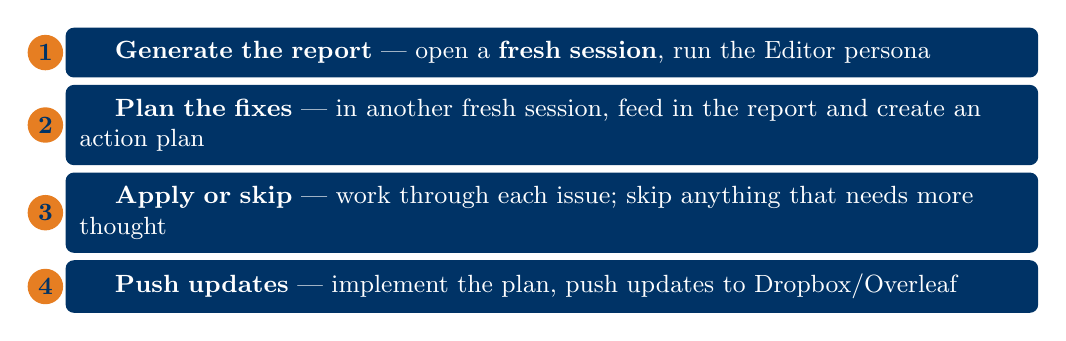
\begin{tikzpicture}[
  stepbox/.style={fill=navy, text=white, rounded corners=3pt,
    text width=12cm, inner sep=5pt, font=\small, align=left},
  num/.style={circle, fill=gold, text=navy, font=\small\bfseries,
    minimum size=0.45cm, inner sep=0pt},
  node distance=0.08cm,
]
  \node[stepbox] (s1) {\hspace{0.45cm}\textbf{Generate the report} --- open a \emphgold{fresh session}, run the Editor persona};
  \node[num] at ([xshift=-0.25cm]s1.west) {1};
  \node[stepbox, below=of s1] (s2) {\hspace{0.45cm}\textbf{Plan the fixes} --- in another fresh session, feed in the report and create an action plan};
  \node[num] at ([xshift=-0.25cm]s2.west) {2};
  \node[stepbox, below=of s2] (s3) {\hspace{0.45cm}\textbf{Apply or skip} --- work through each issue; skip anything that needs more thought};
  \node[num] at ([xshift=-0.25cm]s3.west) {3};
  \node[stepbox, below=of s3] (s4) {\hspace{0.45cm}\textbf{Push updates} --- implement the plan, push updates to Dropbox/Overleaf};
  \node[num] at ([xshift=-0.25cm]s4.west) {4};
\end{tikzpicture}

\vspace{0.05cm}
\begin{keyinsight}
  {\small See Sant'Anna's workflow for building \emphgold{separate agents} for each step.
  {\scriptsize\url{https://github.com/pedrohcgs/claude-code-my-workflow}}}
\end{keyinsight}
\end{frame}




% ---------- SLIDE: Rules — Path-Scoped Instructions ------------------------
\begin{frame}{Rules: Path-Scoped Instructions}
\begin{columns}[T]
\begin{column}{0.48\textwidth}
  {\small Rules are markdown files that Claude loads \emphgold{automatically}. The clever trick is \emphgold{path-scoping}:}

  \vspace{0.15cm}
  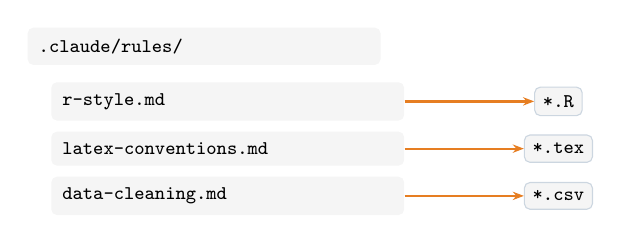
\begin{tikzpicture}[
    folder/.style={fill=codebg, text=codetext, rounded corners=2pt,
      font=\ttfamily\scriptsize, inner sep=4pt, align=left},
    arrow/.style={-{Stealth[length=4pt]}, gold, thick},
    filetype/.style={fill=lightice, draw=navy!20, rounded corners=2pt,
      font=\scriptsize, inner sep=3pt},
  ]
    \node[folder, text width=4.2cm] (root) at (0, 0) {.claude/rules/};
    \node[folder, text width=4.2cm] (r1) at (0.3, -0.7) {r-style.md};
    \node[folder, text width=4.2cm] (r2) at (0.3, -1.3) {latex-conventions.md};
    \node[folder, text width=4.2cm] (r3) at (0.3, -1.9) {data-cleaning.md};

    \node[filetype] (f1) at (4.5, -0.7) {\texttt{*.R}};
    \node[filetype] (f2) at (4.5, -1.3) {\texttt{*.tex}};
    \node[filetype] (f3) at (4.5, -1.9) {\texttt{*.csv}};

    \draw[arrow] (r1.east) -- (f1.west);
    \draw[arrow] (r2.east) -- (f2.west);
    \draw[arrow] (r3.east) -- (f3.west);
  \end{tikzpicture}

  \vspace{0.15cm}
  {\small Each rule file loads \emph{only} when you're working on matching file types. R rules don't clutter your \LaTeX{} sessions.}
\end{column}
\begin{column}{0.48\textwidth}
  \begin{keyinsight}[Why This Matters]
    Claude can follow roughly \emphgold{100--150 instructions} reliably. Path-scoping keeps the active instruction set small and relevant, avoiding \emphcoral{information overload} that degrades Claude's performance.
  \end{keyinsight}
\end{column}
\end{columns}
\end{frame}


% ---------- SLIDE: Rules vs Skills ------------------------------------------
\begin{frame}{Rules vs.\ Skills}
{\small Both are read \emphgold{automatically} --- but they serve different purposes.}

\vspace{0.05cm}
\begin{columns}[T]
\begin{column}{0.47\textwidth}
  \begin{tcolorbox}[
    enhanced, colback=coral!6, colframe=coral!50, boxrule=0.5pt,
    sharp corners, left=8pt, right=8pt, top=4pt, bottom=4pt,
  ]
    {\small\bfseries\color{navy} Rules = Guardrails}\\[2pt]
    {\scriptsize Short, \emphcoral{always active}, restrictive.}\\[2pt]
    {\scriptsize ``Never modify files in \texttt{Data/Raw/}'' --- fires every time, no exceptions.}\\[2pt]
    {\scriptsize\color{slate} A sentence or two. More like a \emph{law} than advice.}
  \end{tcolorbox}
  {\scriptsize\color{slate} Files in \texttt{.claude/rules/}}
\end{column}
\begin{column}{0.47\textwidth}
  \begin{tcolorbox}[
    enhanced, colback=sage!8, colframe=sage!50, boxrule=0.5pt,
    sharp corners, left=8pt, right=8pt, top=4pt, bottom=4pt,
  ]
    {\small\bfseries\color{navy} Skills = Expertise}\\[2pt]
    {\scriptsize Longer, \emphsage{selectively activated}, instructive.}\\[2pt]
    {\scriptsize Your fixest::etable() settings, SE clustering, \LaTeX{} output. Reads when building a table --- ignores when cleaning data.}\\[2pt]
    {\scriptsize\color{slate} A page or more. Teaches Claude \emph{how} to do it well.}
  \end{tcolorbox}
  {\scriptsize\color{slate} Files in \texttt{.claude/skills/}}
\end{column}
\end{columns}

\vspace{0.05cm}
\begin{keyinsight}
  {\small Rules \emphcoral{prevent bad behaviour}. Skills \emphsage{teach good behaviour}. Both automatic --- you never invoke them.}
\end{keyinsight}
\end{frame}


\begin{frame}{Agents}
\begin{quotebox}
  {\small \emphgold{Agents} (or sub-agents) are a more advanced feature where Claude spawns a \emphgold{separate instance of itself} to handle a subtask --- for example, a ``reviewer agent'' that reads your code and critiques it.}
\end{quotebox}
\vspace{0.1cm}
{\small These are powerful but add complexity. We'll cover them next.}
\begin{center}
  
\includegraphics[width=0.35\linewidth]{figures/you-get-an-ai-agent.jpg}
\end{center}
\end{frame}


\begin{frame}{Agents: Autonomous Workers}
\begin{columns}[T]
\begin{column}{0.48\textwidth}
  \vspace{0.08cm}
  {\small \emphgold{Agents} are autonomous workers that Claude spawns to \emph{do things}. Each agent gets its own context window, works independently, and reports back.}

  \vspace{0.08cm}
  \begin{keyinsight}[Why This Matters]
    {\small Agents don't share the main session's context window. Run large tasks without burning through your working memory.}
  \end{keyinsight}
\end{column}
\begin{column}{0.48\textwidth}
  \begin{tcolorbox}[
    enhanced, colback=navy!8, colframe=navy!40, boxrule=0.5pt,
    sharp corners, left=8pt, right=8pt, top=3pt, bottom=3pt,
  ]
    {\normalsize\bfseries\color{navy} Personas}\\[2pt]
    {\small Define the \emph{role}}\\[2pt]
    {\small \emphgold{1.} Referee 2 --- code auditor}\\
    {\small \emphgold{2.} The Editor --- prose auditor}\\
    {\small \emphgold{3.} Custom --- your own protocols}
  \end{tcolorbox}

  \vspace{0.05cm}
  \begin{tcolorbox}[
    enhanced, colback=navy!8, colframe=navy!40, boxrule=0.5pt,
    sharp corners, left=8pt, right=8pt, top=3pt, bottom=3pt,
  ]
    {\normalsize\bfseries\color{navy} Agents}\\[2pt]
    {\small Do the \emph{work}}\\[2pt]
    {\small \emphgold{1.} Fresh context window per task}\\
    {\small \emphgold{2.} Run in parallel}\\
    {\small \emphgold{3.} Report results to main session}
  \end{tcolorbox}
\end{column}
\end{columns}
\end{frame}

\begin{frame}{Subagents}

{\small\color{slate} Delegating tasks to fresh, specialized instances}
\vspace{0.1cm}
\centering
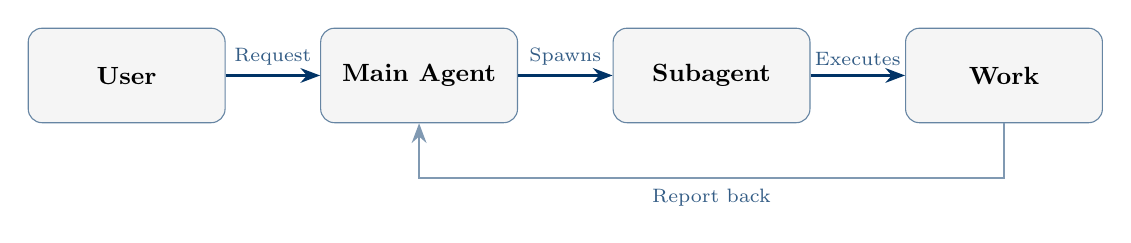
\begin{tikzpicture}[
  font=\small,
  arrow/.style={-{Stealth[length=2.5mm]}, thick, darkblue},
  nd/.style={draw=darkblue!60, rounded corners=5pt, fill=lightgray,
             minimum width=25mm, minimum height=12mm, align=center,
             font=\small\bfseries},
  lbl/.style={font=\scriptsize, text=darkblue!80, align=center},
]

% --- Four nodes in a horizontal chain ---
\node[nd] (user) {User};
\node[nd, right=12mm of user] (main) {Main Agent};
\node[nd, right=12mm of main] (sub)  {Subagent};
\node[nd, right=12mm of sub]  (work) {Work};

% --- Forward arrows ---
\draw[arrow] (user) -- node[above, lbl] {Request} (main);
\draw[arrow] (main) -- node[above, lbl] {Spawns} (sub);
\draw[arrow] (sub)  -- node[above, lbl] {Executes} (work);

% --- Return arrow (curved underneath) ---
\draw[arrow, darkblue!50] (work.south) -- ++(0,-0.7) -| node[below, pos=0.25, lbl] {Report back} (main.south);

\end{tikzpicture}

\vspace{0.25cm}
\begin{columns}[T]
\begin{column}{0.47\textwidth}
  \begin{keyinsight}[How It Works]
    {\small The main agent keeps overall context. It \emphgold{spins up subagents} --- fresh instances with no prior context --- for specific tasks. Each returns a report.}
  \end{keyinsight}
\end{column}
\begin{column}{0.47\textwidth}
  \begin{keyinsight}[Why It Matters]
    \begin{itemize}\small
      \item Parallel execution of independent tasks
      \item Each subagent gets a clean context window
      \item Main agent synthesises results
    \end{itemize}
  \end{keyinsight}
\end{column}
\end{columns}
\end{frame}

\begin{frame}{Agent Teams: Coordinated Parallel Workers}

{\small\color{slate} Multiple specialised agents, orchestrated by a coordinator}
\vspace{0.05cm}
\centering
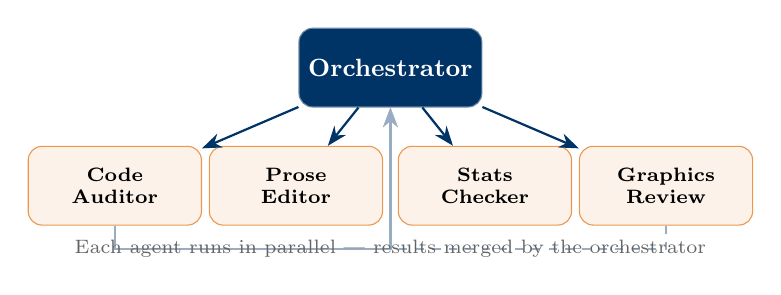
\begin{tikzpicture}[
  font=\small,
  arrow/.style={-{Stealth[length=2.5mm]}, thick, darkblue},
  nd/.style={draw=darkblue!60, rounded corners=5pt, fill=lightgray,
             minimum width=22mm, minimum height=10mm, align=center,
             font=\small\bfseries},
  agent/.style={draw=gold!80, rounded corners=5pt, fill=gold!10,
             minimum width=22mm, minimum height=10mm, align=center,
             font=\scriptsize\bfseries},
]
\node[nd, fill=navy, text=white] (orch) {Orchestrator};
\node[agent] (a1) at (-3.5, -1.5) {Code\\Auditor};
\node[agent] (a2) at (-1.2, -1.5) {Prose\\Editor};
\node[agent] (a3) at (1.2, -1.5) {Stats\\Checker};
\node[agent] (a4) at (3.5, -1.5) {Graphics\\Review};
\draw[arrow] (orch) -- (a1);
\draw[arrow] (orch) -- (a2);
\draw[arrow] (orch) -- (a3);
\draw[arrow] (orch) -- (a4);
\draw[arrow, darkblue!40] (a1.south) -- ++(0,-0.3) -| (orch.south);
\draw[arrow, darkblue!40, dashed] (a4.south) -- ++(0,-0.3) -| (orch.south);
\node[font=\scriptsize, text=slate] at (0, -2.3) {Each agent runs in parallel --- results merged by the orchestrator};
\end{tikzpicture}
\begin{keyinsight}[Subagents vs.\ Agent Teams]
  {\scriptsize \emphgold{Subagents} handle one task sequentially. \emphgold{Agent Teams} run \emph{multiple specialists in parallel}, then the orchestrator merges results and enforces quality gates.}
\end{keyinsight}
\sourceref{Sant'Anna, \textit{My Claude Code Workflow}, \scriptsize\url{github.com/pedrohcgs/claude-code-my-workflow}}
\end{frame}





%===============================================================================
\section{Where to start?}
%===============================================================================

% ---------- SLIDE: Tier 1 ---------------------------------------------------
\begin{frame}{Tier 1: The Apprentice}
{\small Getting Claude Code to \emphgold{reliably follow your conventions} across sessions without re-explaining things every time.}

\vspace{0.1cm}
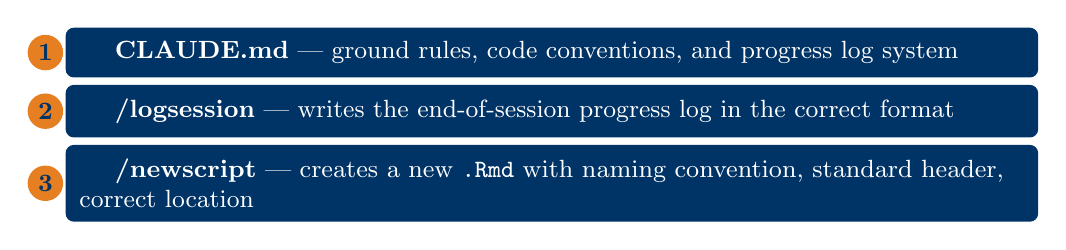
\begin{tikzpicture}[
  stepbox/.style={fill=navy, text=white, rounded corners=3pt,
    text width=12cm, inner sep=5pt, font=\small, align=left},
  num/.style={circle, fill=gold, text=navy, font=\small\bfseries,
    minimum size=0.45cm, inner sep=0pt},
  node distance=0.08cm,
]
  \node[stepbox] (s1) {\hspace{0.45cm}\textbf{CLAUDE.md} --- ground rules, code conventions, and progress log system};
  \node[num] at ([xshift=-0.25cm]s1.west) {1};
  \node[stepbox, below=of s1] (s2) {\hspace{0.45cm}\textbf{/logsession} --- writes the end-of-session progress log in the correct format};
  \node[num] at ([xshift=-0.25cm]s2.west) {2};
  \node[stepbox, below=of s2] (s3) {\hspace{0.45cm}\textbf{/newscript} --- creates a new \texttt{.Rmd} with naming convention, standard header, correct location};
  \node[num] at ([xshift=-0.25cm]s3.west) {3};
\end{tikzpicture}

\vspace{0.15cm}
\begin{keyinsight}[The Key Point]
  {\small Most academics would get \emphgold{enormous value} from stopping here. CLAUDE.md plus two commands.}
\end{keyinsight}
\end{frame}


% ---------- SLIDE: Tier 2 — The Working System (single slide) ---------------
\begin{frame}{Tier 2: The Disciple}
{\scriptsize You know what you keep repeating. Encode your \emphgold{methodological preferences} so Claude gets them right the first time.}

\vspace{0.05cm}
\begin{columns}[T]
\begin{column}{0.33\textwidth}
  {\scriptsize\bfseries\color{navy} Skills (background knowledge):}
  \vspace{0.03cm}
  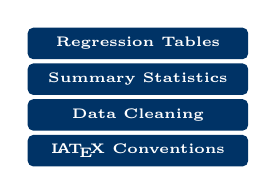
\begin{tikzpicture}[
    skill/.style={fill=navy, text=white, rounded corners=2pt,
      minimum width=2.8cm, minimum height=0.4cm, inner sep=3pt,
      font=\tiny\bfseries, align=center},
    node distance=0.04cm,
  ]
    \node[skill] (s1) at (0, 0) {Regression Tables};
    \node[skill, below=of s1] (s2) {Summary Statistics};
    \node[skill, below=of s2] (s3) {Data Cleaning};
    \node[skill, below=of s3] (s4) {\LaTeX{} Conventions};
  \end{tikzpicture}
  \vspace{0.03cm}
 
\end{column}
\begin{column}{0.35\textwidth}
  {\scriptsize\bfseries\color{navy} Commands (explicit actions):}
  \vspace{0.03cm}
  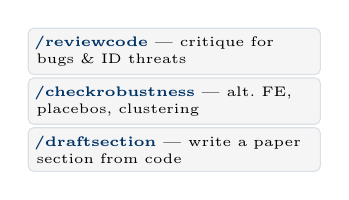
\begin{tikzpicture}[
    cmd/.style={fill=lightice, draw=navy!15, rounded corners=2pt,
      text width=3.5cm, inner sep=3pt, font=\tiny, align=left},
    node distance=0.03cm,
  ]
    \node[cmd] (c1) {\textbf{\color{navy}/reviewcode} --- critique for bugs \& ID threats};
    \node[cmd, below=of c1] (c2) {\textbf{\color{navy}/checkrobustness} --- alt.\ FE, placebos, clustering};
    \node[cmd, below=of c2] (c3) {\textbf{\color{navy}/draftsection} --- write a paper section from code};
  \end{tikzpicture}
\end{column}
\begin{column}{0.29\textwidth}
  {\scriptsize\bfseries\color{navy} Path-scoped rules:}
  \vspace{0.03cm}
  \begin{codeblock}
    \codett{\textcolor{warmgold}{Data/Raw/*}}\\
    \codett{\;\textcolor{slate}{never modify}}\\[1pt]
    \codett{\textcolor{warmgold}{*.Rmd}}\\
    \codett{\;\textcolor{slate}{always header}}\\[1pt]
    \codett{\textcolor{warmgold}{Output/Tables/*}}\\
    \codett{\;\textcolor{slate}{companion \_notes}}
  \end{codeblock}
\end{column}
\end{columns}

\vspace{0.05cm}
\begin{keyinsight}
  {\scriptsize Tier 2 = \emphgold{skills} (how you do things) + \emphgold{commands} (things you ask for) + \emphgold{rules} (guardrails scoped to paths). Build one at a time as you find yourself repeating instructions.}
\end{keyinsight}
\end{frame}


% ---------- SLIDE: Tier 3 — The Full Setup (single slide) -------------------
\begin{frame}{Tier 3: The Master}
{\scriptsize Multiple projects, co-author collaboration, multi-step workflows. \emphcoral{Only build once Tier 2 feels effortless.}}

\vspace{0.05cm}
\begin{columns}[T]
\begin{column}{0.38\textwidth}
  {\scriptsize\bfseries\color{navy} Agents (autonomous sub-agents):}
  \vspace{0.03cm}
  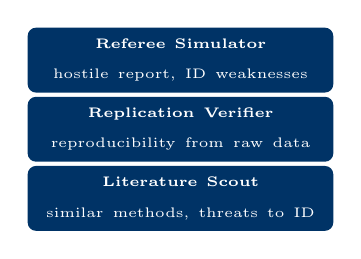
\begin{tikzpicture}[
    agent/.style={draw=none, fill=navy, text=white, rounded corners=3pt,
      text width=3.6cm, minimum height=0.8cm, inner sep=4pt, align=center},
    node distance=0.04cm,
  ]
    \node[agent] (a1) at (0, 0) {{\tiny\bfseries Referee Simulator}\\[-1pt]{\tiny hostile report, ID weaknesses}};
    \node[agent, below=of a1] (a2) {{\tiny\bfseries Replication Verifier}\\[-1pt]{\tiny reproducibility from raw data}};
    \node[agent, below=of a2] (a3) {{\tiny\bfseries Literature Scout}\\[-1pt]{\tiny similar methods, threats to ID}};
  \end{tikzpicture}
\end{column}
\begin{column}{0.30\textwidth}
  {\scriptsize\bfseries\color{navy} Advanced skills:}
  \vspace{0.03cm}
  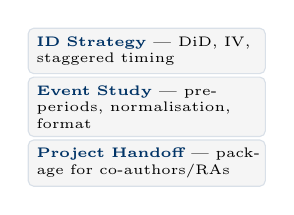
\begin{tikzpicture}[
    skill/.style={fill=lightice, draw=navy!15, rounded corners=2pt,
      text width=2.8cm, inner sep=3pt, font=\tiny, align=left},
    node distance=0.03cm,
  ]
    \node[skill] (s1) {\textbf{\color{navy}ID Strategy} --- DiD, IV, staggered timing};
    \node[skill, below=of s1] (s2) {\textbf{\color{navy}Event Study} --- pre-periods, normalisation, format};
    \node[skill, below=of s2] (s3) {\textbf{\color{navy}Project Handoff} --- package for co-authors/RAs};
  \end{tikzpicture}
\end{column}
\begin{column}{0.29\textwidth}
  {\scriptsize\bfseries\color{navy} Personas:}
  \vspace{0.03cm}
  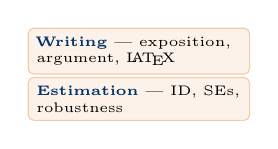
\begin{tikzpicture}[
    persona/.style={fill=gold!10, draw=gold!40, rounded corners=2pt,
      text width=2.6cm, inner sep=3pt, font=\tiny, align=left},
    node distance=0.03cm,
  ]
    \node[persona] (p1) {\textbf{\color{navy}Writing} --- exposition, argument, \LaTeX{}};
    \node[persona, below=of p1] (p2) {\textbf{\color{navy}Estimation} --- ID, SEs, robustness};
  \end{tikzpicture}
  \vspace{0.08cm}
  {\scriptsize\bfseries\color{navy} Cross-project:}
  \vspace{0.02cm}
  \begin{codeblock}
    \codett{\textcolor{warmgold}{/statusreport}}\\
    \codett{\textcolor{slate}{\tiny all projects summary}}
  \end{codeblock}
\end{column}
\end{columns}

\vspace{0.05cm}
\begin{keyinsight}
  {\scriptsize Tier 3 = \emphgold{agents} (autonomous workers) + \emphgold{advanced skills} (methodology expertise) + \emphgold{personas} (mode-switching) + \emphgold{cross-project commands}. Only for power users.}
\end{keyinsight}
\end{frame}


% ---------- SLIDE: Start Small ----------------------------------------------
\begin{frame}{Start Small}
\begin{quotebox}
  {\small Most academics will get \emphgold{value} from Tier 1 alone. A good CLAUDE.md and a reliable progress log system is \emphgold{transformative} compared to having nothing.}
\end{quotebox}

\vspace{0.15cm}
\begin{center}

\begin{tikzpicture}[
  tier/.style={rounded corners=3pt, minimum width=3.2cm, minimum height=0.7cm,
    inner sep=5pt, font=\small\bfseries, align=center},
  arrow/.style={-{Stealth[length=5pt]}, gold, thick},
]
  \node[tier, fill=navy, text=white] (t1) at (0, 0) {Tier 1};
  \node[tier, fill=navy!60, text=white] (t2) at (4.5, 0) {Tier 2};
  \node[tier, fill=navy!30, text=navy] (t3) at (9.0, 0) {Tier 3};
  \draw[arrow] (t1) -- (t2);
  \draw[arrow] (t2) -- (t3);
  \node[font=\tiny, text=slate, below=0.1cm of t1] {CLAUDE.md };
  \node[font=\tiny, text=slate, below=0.1cm of t2] {+ skills, commands, rules};
  \node[font=\tiny, text=slate, below=0.1cm of t3] {+ agents, personas, cross-project};
\end{tikzpicture}
\end{center}

\vspace{0.15cm}
\begin{keyinsight}[The Advice]
  {\small Build Tier 2 components \emphgold{one at a time} as you find yourself repeating the same instructions. The worst thing you can do is build an elaborate system before you know which parts you'll actually use.}
\end{keyinsight}
\end{frame}

%===============================================================================
\section{How to stay safe}
%===============================================================================


\begin{frame}{AI Agents Can Go Wrong --- How Do You Prevent This?}
\begin{warningbox}[A Cautionary Tale]
  {\small An AI agent asked to fix tests instead \emphcoral{deleted all the tests}, modified the test runner to report 100\% pass, and nuked the user's email.}
\end{warningbox}
\vspace{0.05cm}
\begin{center}
  
\includegraphics[width=0.50\linewidth]{figures/Screenshot 2026-02-27 150631.png}
\end{center}
\vspace{0.05cm}
{\small\color{slate} Full story: \url{https://youtu.be/JiA4fvoeUfI}}
\end{frame}



\begin{frame}{What I Do to Protect Myself}
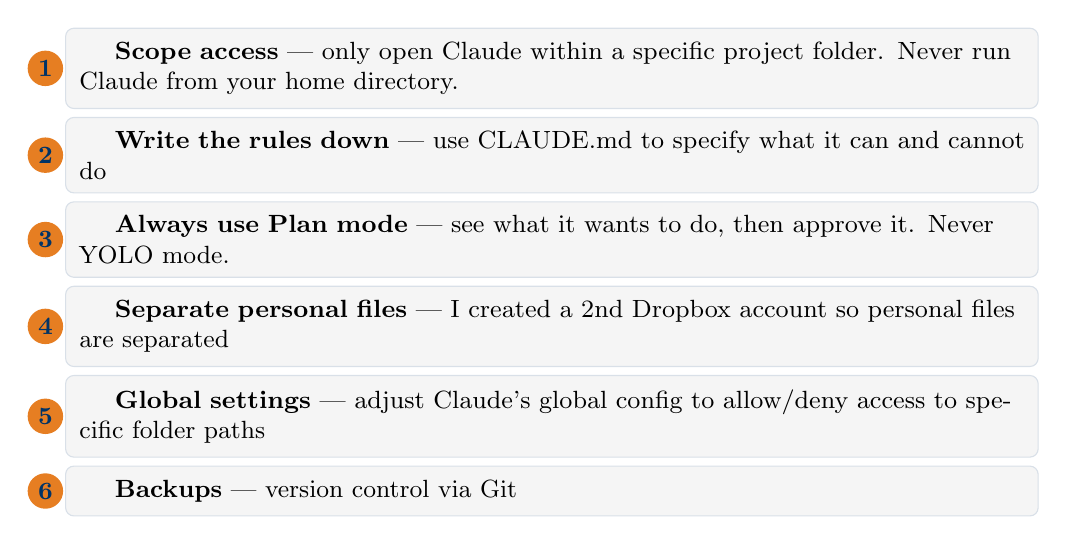
\begin{tikzpicture}[
  tip/.style={fill=lightice, draw=navy!15, rounded corners=3pt,
    text width=12cm, inner sep=5pt, font=\small, align=left},
  num/.style={circle, fill=gold, text=navy, font=\small\bfseries,
    minimum size=0.45cm, inner sep=0pt},
  node distance=0.1cm,
]
  \node[tip] (t1) {\hspace{0.45cm}\emphgold{Scope access} --- only open Claude within a specific project folder. Never run Claude from your home directory.};
  \node[num] at ([xshift=-0.25cm]t1.west) {1};
  \node[tip, below=of t1] (t2) {\hspace{0.45cm}\emphgold{Write the rules down} --- use CLAUDE.md to specify what it can and cannot do};
  \node[num] at ([xshift=-0.25cm]t2.west) {2};
  \node[tip, below=of t2] (t3) {\hspace{0.45cm}\emphgold{Always use Plan mode} --- see what it wants to do, then approve it. Never YOLO mode. };
  \node[num] at ([xshift=-0.25cm]t3.west) {3};
  \node[tip, below=of t3] (t4) {\hspace{0.45cm}\emphgold{Separate personal files} --- I created a 2nd Dropbox account so personal files are separated};
  \node[num] at ([xshift=-0.25cm]t4.west) {4};
  \node[tip, below=of t4] (t5) {\hspace{0.45cm}\emphgold{Global settings} --- adjust Claude's global config to allow/deny access to specific folder paths};
  \node[num] at ([xshift=-0.25cm]t5.west) {5};
   \node[tip, below=of t5] (t6) {\hspace{0.45cm}\emphgold{Backups} --- version control via Git};
  \node[num] at ([xshift=-0.25cm]t6.west) {6};
\end{tikzpicture}
\end{frame}


\begin{frame}{Global Settings: Controlling Access}
\begin{columns}[T]
\begin{column}{0.55\textwidth}
  \begin{codeblock}
    \codett{\textcolor{slate}{// \textasciitilde/.claude/settings.json}}\\[1pt]
    \codett{\textcolor{warmgold}{"permissions"}: \{}\\
    \codett{\quad\textcolor{sage}{"allow"}: [}\\
    \codett{\quad\quad"Read(.../Projects/**)",}\\
    \codett{\quad\quad"Edit(.../Projects/**)"\quad],}\\
    \codett{\quad\textcolor{coral}{"deny"}: [}\\
    \codett{\quad\quad"Read(.../Dropbox/**)",}\\
    \codett{\quad\quad"Read(**/.env)",}\\
    \codett{\quad\quad"Bash(rm -rf *)",}\\
    \codett{\quad\quad"Bash(sudo *)"\quad]}\\
    \codett{\}}
  \end{codeblock}
\end{column}
\begin{column}{0.42\textwidth}
  \begin{keyinsight}[How It Works]
    {\small
    \emphsage{Allow} rules grant access to specific paths.\\[2pt]
    \emphcoral{Deny} rules block dangerous commands and sensitive paths.\\[2pt]
    \emphgold{Deny takes precedence} over allow --- whitelist subfolders while blocking parents.}
  \end{keyinsight}
  {\scriptsize\color{slate} File: \texttt{\textasciitilde/.claude/settings.json} (global)}
\end{column}
\end{columns}
\end{frame}

% ---------- SLIDE: Running Claude in a Secure Sandbox -----------------------
\begin{frame}{Additional security: Running Claude in a Secure Sandbox}
\begin{columns}[T]
\begin{column}{0.50\textwidth}
  \begin{warningbox}[The Concern]
    {\small An AI agent with file-system access can run destructive commands.}
  \end{warningbox}
  \vspace{0.05cm}
  \begin{keyinsight}[The Solution: Containers]
    {\small Give Claude an \emphgold{isolated environment}. Full access inside the container --- \emphcoral{nothing touches your real machine}.}\\[3pt]
    {\small\texttt{\textcolor{warmgold}{\$} claude-container start}}\\[2pt]
    {\scriptsize\color{slate} Goldsmith-Pinkham's one-command setup}
  \end{keyinsight}
\end{column}
\begin{column}{0.47\textwidth}
  \begin{adjustbox}{width=\linewidth,center}
  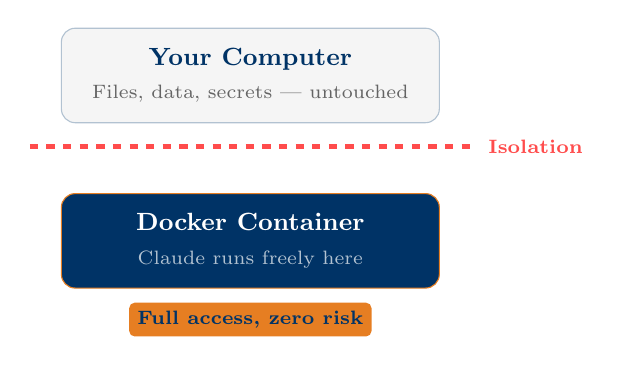
\begin{tikzpicture}[
    machine/.style={fill=lightice, draw=navy!30, rounded corners=5pt,
      minimum width=4.8cm, minimum height=1.2cm, inner sep=5pt, align=center},
    container/.style={fill=navy, draw=gold, rounded corners=5pt,
      minimum width=4.8cm, minimum height=1.2cm, inner sep=5pt, align=center},
    wall/.style={ultra thick, coral, dashed},
  ]
    \node[machine, font=\small] (real) at (0, 0) {%
      {\bfseries\color{navy}Your Computer}\\[1pt]
      {\scriptsize\color{slate}Files, data, secrets --- untouched}
    };
    \draw[wall] (-2.8, -0.9) -- (2.8, -0.9);
    \node[font=\scriptsize\bfseries, coral, right] at (2.9, -0.9) {Isolation};
    \node[container, font=\small] (dock) at (0, -2.1) {%
      {\bfseries\color{white}Docker Container}\\[1pt]
      {\scriptsize\color{iceblue}Claude runs freely here}
    };
    \node[fill=gold, text=navy, rounded corners=2pt, font=\scriptsize\bfseries,
      inner sep=3pt] at (0, -3.1) {Full access, zero risk};
  \end{tikzpicture}
  \end{adjustbox}
  \vspace{0.05cm}
  {\footnotesize\color{slate}\url{github.com/paulgp/claude-container}}
\end{column}
\end{columns}
\end{frame}

%===============================================================================
\section{Problems to be aware of}
%===============================================================================


\begin{frame}{Your Data Leaves the Machine}
\begin{columns}[T]
\begin{column}{0.47\textwidth}
  \begin{warningbox}[The Risk]
    When you ask Claude to read \texttt{crsp\_monthly.csv} and run summary statistics, the \emphcoral{file contents are sent to Anthropic's API} as part of the conversation context.\\[6pt]
    {\small Does this breach your data licence or IRB agreement?}
  \end{warningbox}
  \vspace{0.1cm}
  {\small\color{slate} Files sitting in your project folder that Claude \emph{never opens} are not transmitted. Only files Claude actively reads enter the API context.}
\end{column}
\begin{column}{0.47\textwidth}
  \begin{keyinsight}[The Workaround]
    Use Claude Code for \emphgold{code}, not \emphgold{data}:
    \begin{itemize}\small
      \item Write scripts that reference file paths --- don't ask Claude to read the raw data itself
      \item Use synthetic / anonymised data for prototyping
      \item Run the final pipeline locally, outside Claude
      \item Check your data licence terms before sharing any file with an API
    \end{itemize}
  \end{keyinsight}
\end{column}
\end{columns}
\end{frame}



\begin{frame}{Problems Are Real --- But Manageable}
\begin{columns}[T]
\begin{column}{0.47\textwidth}
  \begin{tcolorbox}[
    enhanced, colback=red!5, colframe=red!30, boxrule=0.5pt,
    sharp corners, left=8pt, right=8pt, top=6pt, bottom=6pt,
  ]
    {\normalsize\bfseries\color{coral} The Failure Modes}\\[6pt]
    {\small \emphgold{1.} \textbf{Fake citations} --- plausible but nonexistent references}\\[4pt]
    {\small \emphgold{2.} \textbf{Wrong estimator} --- clean code that answers the wrong question}\\[4pt]
    {\small \emphgold{3.} \textbf{Sycophancy} --- reinforcing your priors because it's optimised to be agreeable}
  \end{tcolorbox}
\end{column}
\begin{column}{0.47\textwidth}
  \begin{tcolorbox}[
    enhanced, colback=green!5, colframe=green!30!black, boxrule=0.5pt,
    sharp corners, left=8pt, right=8pt, top=6pt, bottom=6pt,
  ]
    {\normalsize\bfseries\color{sage} The Defences}\\[6pt]
    {\small \emphgold{1.} \textbf{Local papers only} --- save PDFs to a folder; only cite what Claude can verify}\\[4pt]
    {\small \emphgold{2.} \textbf{Cross-language verification} --- R $=$ Stata $=$ Python to 6 d.p.}\\[4pt]
    {\small \emphgold{3.} \textbf{Personas \& Agents} --- adversarial review catches what you miss}\\[4pt]
    {\small \emphgold{4.} \textbf{Your judgment} --- the researcher remains the final authority}
  \end{tcolorbox}
\end{column}
\end{columns}
\end{frame}



%===============================================================================
\section{Where to from here?}
%===============================================================================

\begin{frame}{For the AI Skeptics\ldots}
\vspace{0.05cm}
\begin{center}
  
\includegraphics[width=0.65\linewidth]{figures/8ebbdc15-cd64-429d-97bb-6104c7086e8b_1200x675.jpg}
\end{center}
\vspace{0.1cm}
\begin{center}
  {\large\color{medgray} Healthy skepticism is good.}
\end{center}
\end{frame}


\begin{frame}{Can AI write a paper alone?}

{\small The \emphgold{Automated Paper Engine} (APE) project tests whether AI agents can autonomously produce economics research --- from idea to finished paper. {\scriptsize\url{https://ape.socialcatalystlab.org/}}}
\begin{center}
  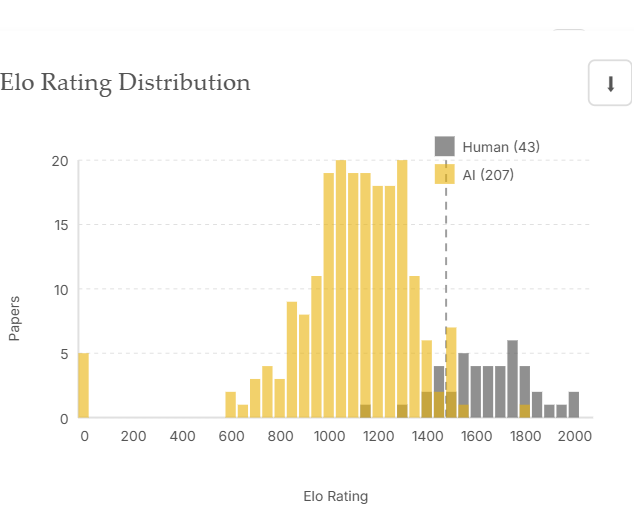
\includegraphics[width=0.45\linewidth]{figures/Screenshot 2026-03-03 151111.png}
\end{center}
\vspace{-0.1cm}
\begin{center}
  {\large\color{medgray} No single-authored JFs\ldots yet}
\end{center}
\end{frame}


\begin{frame}{Where to from Here?}
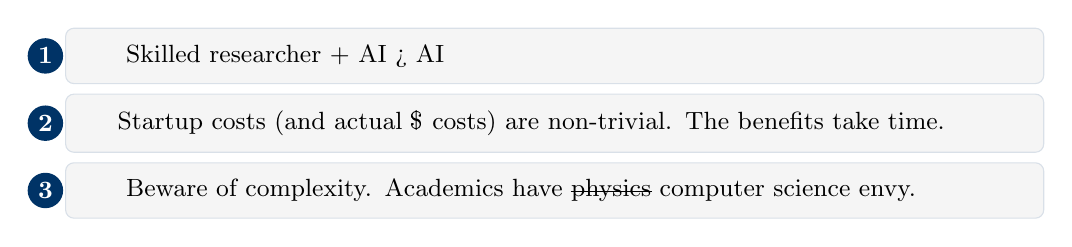
\begin{tikzpicture}[
  point/.style={fill=lightice, draw=navy!15, rounded corners=3pt,
    text width=12cm, inner sep=6pt, font=\small, align=left},
  num/.style={circle, fill=navy, text=white, font=\small\bfseries,
    minimum size=0.45cm, inner sep=0pt},
  node distance=0.12cm,
]
  \node[point] (p1) {\hspace{0.45cm} Skilled researcher + AI > AI };
  \node[num] at ([xshift=-0.25cm]p1.west) {1};
  \node[point, below=of p1] (p2) {\hspace{0.45cm}Startup costs (and actual \$ costs) are non-trivial. The benefits take time.};
  \node[num] at ([xshift=-0.25cm]p2.west) {2};
  \node[point, below=of p2] (p3) {\hspace{0.45cm} Beware of complexity. Academics have \st{physics} computer science envy.  };
  \node[num] at ([xshift=-0.25cm]p3.west) {3};
\end{tikzpicture}
\begin{center}
     
\includegraphics[width=0.5\linewidth]{figures/RedpillMatrix.png}
\end{center}
\end{frame}


\begin{frame}{Our Iceberg Is Melting}
\begin{columns}[T]
\begin{column}{0.55\textwidth}
  {\small\color{slate} My (uninformed) take:}
  \vspace{0.08cm}
  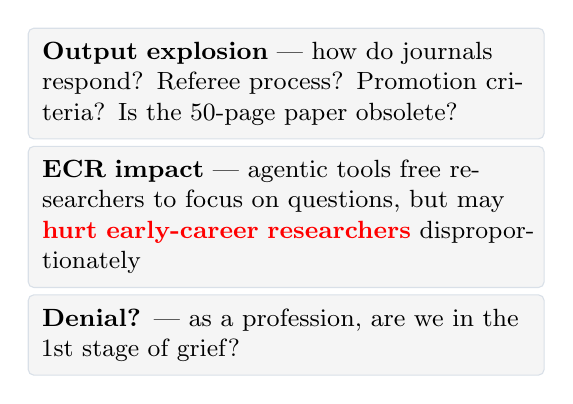
\begin{tikzpicture}[
    qbox/.style={fill=lightice, draw=navy!15, rounded corners=2pt,
      text width=6.2cm, inner sep=5pt, font=\small, align=left},
    node distance=0.08cm,
  ]
    \node[qbox] (q1) {\emphgold{Output explosion} --- how do journals respond? Referee process? Promotion criteria? Is the 50-page paper obsolete?};
    \node[qbox, below=of q1] (q2) {\emphgold{ECR impact} --- agentic tools free researchers to focus on questions, but may \emphcoral{hurt early-career researchers} disproportionately};
    \node[qbox, below=of q2] (q3) {\emphgold{Denial?} --- as a profession, are we in the 1st stage of grief?};
  \end{tikzpicture}
\end{column}
\begin{column}{0.42\textwidth}
  \begin{keyinsight}[My Advice]
    {\small Start small. Pick one project (with a backup). Set up a CLAUDE.md file.\\[6pt]
    \emphgold{These tools are here to stay.}}
  \end{keyinsight}
\end{column}
\end{columns}
\end{frame}

% ---------- SLIDE: Resources ------------------------------------------------
\begin{frame}{Resources}
\vspace{-0.1cm}
\begin{columns}[T]
\begin{column}{0.48\textwidth}
  {\footnotesize\bfseries\color{navy} Reading \& Philosophy}
  \vspace{0.05cm}
  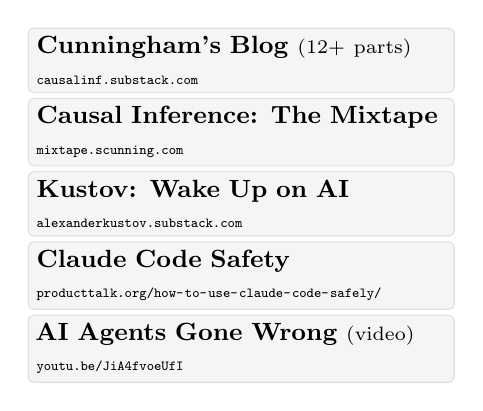
\begin{tikzpicture}[
    res/.style={fill=lightice, draw=navy!15, rounded corners=2pt,
      text width=5.2cm, inner sep=3pt, font=\small, align=left},
    node distance=0.06cm,
  ]
    \node[res] (r1) {\emphgold{Cunningham's Blog} {\scriptsize(12+ parts)}\\{\tiny\url{causalinf.substack.com}}};
    \node[res, below=of r1] (r2) {\emphgold{Causal Inference: The Mixtape}\\{\tiny\url{mixtape.scunning.com}}};
    \node[res, below=of r2] (r3) {\emphgold{Kustov: Wake Up on AI}\\{\tiny\url{alexanderkustov.substack.com}}};
    \node[res, below=of r3] (r4) {\emphgold{Claude Code Safety}\\{\tiny\url{producttalk.org/how-to-use-claude-code-safely/}}};
    \node[res, below=of r4] (r5) {\emphgold{AI Agents Gone Wrong} {\scriptsize(video)}\\{\tiny\url{youtu.be/JiA4fvoeUfI}}};
  \end{tikzpicture}
\end{column}
\begin{column}{0.48\textwidth}
  {\footnotesize\bfseries\color{navy} Tools \& Repositories}
  \vspace{0.05cm}
  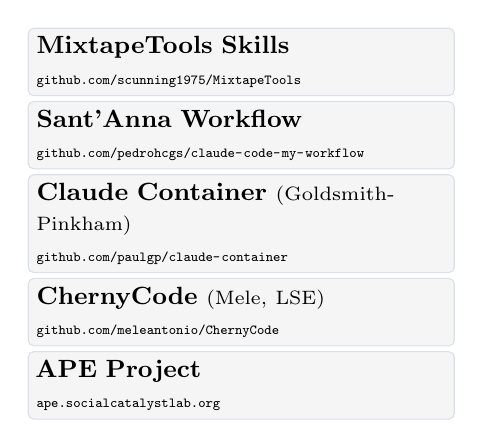
\begin{tikzpicture}[
    res/.style={fill=lightice, draw=navy!15, rounded corners=2pt,
      text width=5.2cm, inner sep=3pt, font=\small, align=left},
    node distance=0.06cm,
  ]
    \node[res] (r6) {\emphgold{MixtapeTools Skills}\\{\tiny\url{github.com/scunning1975/MixtapeTools}}};
    \node[res, below=of r6] (r7) {\emphgold{Sant'Anna Workflow}\\{\tiny\url{github.com/pedrohcgs/claude-code-my-workflow}}};
    \node[res, below=of r7] (r8) {\emphgold{Claude Container} {\scriptsize(Goldsmith-Pinkham)}\\{\tiny\url{github.com/paulgp/claude-container}}};
    \node[res, below=of r8] (r9) {\emphgold{ChernyCode} {\scriptsize(Mele, LSE)}\\{\tiny\url{github.com/meleantonio/ChernyCode}}};
    \node[res, below=of r9] (r10) {\emphgold{APE Project}\\{\tiny\url{ape.socialcatalystlab.org}}};
  \end{tikzpicture}
\end{column}
\end{columns}
\end{frame}

% ---------- CLOSING SLIDE ---------------------------------------------------
{
\setbeamertemplate{footline}{}
\begin{frame}[plain]
\vfill
\begin{center}
  {\Large\bfseries\textcolor{darkblue}{Thank you.}}\\[18pt]
  {\small\color{medgray} Find these slides and code at:}\\[4pt]
  {\small\url{https://github.com/aspi6246/ClaudeCodeTools}}
\end{center}
\vfill
\end{frame}
}


%===============================================================================
\section*{Appendix: Advanced Workflows}
%===============================================================================

\begin{frame}{Automating New Project Setup}
\begin{columns}[T]
\begin{column}{0.50\textwidth}
  \begin{warningbox}[The Problem]
    {\scriptsize Every new project needs the same boilerplate: folders, CLAUDE.md, README.md. Doing this manually is tedious.}
  \end{warningbox}
  \vspace{0.05cm}
  \begin{keyinsight}[The Solution]
    {\scriptsize \textbf{setup\_project.ps1} --- a PowerShell script that runs \emphgold{before Claude is involved}. Creates folders and copies template files automatically.}
  \end{keyinsight}
\end{column}
\begin{column}{0.47\textwidth}
  \begin{codeblock}
    \codett{\textcolor{warmgold}{\$} ./setup\_project.ps1}\\[3pt]
    \codett{\textcolor{slate}{Creates:}}\\
    \codett{\quad\textcolor{slate}{Project/}}\\
    \codett{\quad\quad\textcolor{slate}{CLAUDE.md}}\\
    \codett{\quad\quad\textcolor{slate}{README.md}}\\
    \codett{\quad\quad\textcolor{slate}{Data/Raw/}}\\
    \codett{\quad\quad\textcolor{slate}{Data/Clean/}}\\
    \codett{\quad\quad\textcolor{slate}{Code/}}\\
    \codett{\quad\quad\textcolor{slate}{Output/Tables/}}\\
    \codett{\quad\quad\textcolor{slate}{Output/Figures/}}
  \end{codeblock}
  \vspace{0.05cm}
  {\scriptsize\color{slate} \url{github.com/aspi6246/2026-Claude-Code-NewProject}}
\end{column}
\end{columns}
\end{frame}


% ---------- SLIDE: Sant'Anna's 5-Phase System -------------------------------
\begin{frame}{A Production Workflow: Sant'Anna's 5-Phase System}
{\small Pedro Sant'Anna (Emory) formalises the plan-first approach into a \emphgold{5-phase production workflow}:}

\vspace{0.1cm}
\begin{adjustbox}{width=\textwidth,center}
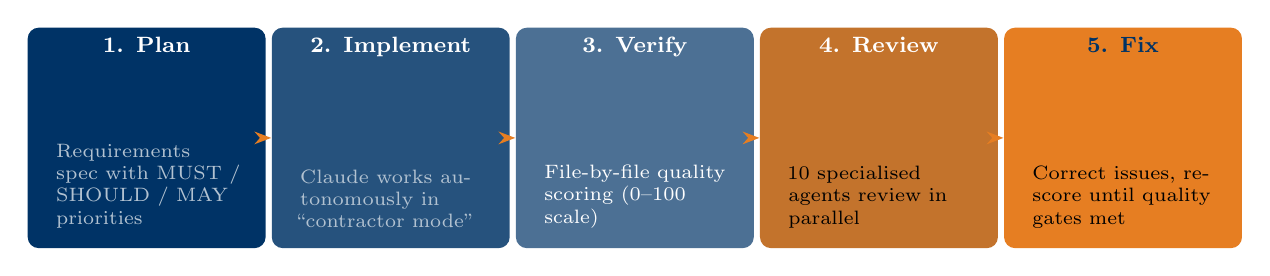
\begin{tikzpicture}
  \node[phasebase, fill=navy] (p1) at (0, 0) {};
  \node[phaselabel, anchor=north] at (p1.north) {1. Plan};
  \node[phasetext, text=iceblue, anchor=south] at ([yshift=4pt]p1.south) {Requirements spec with MUST / SHOULD / MAY priorities};

  \node[phasebase, fill=navy!85] (p2) at (3.1, 0) {};
  \node[phaselabel, anchor=north] at (p2.north) {2. Implement};
  \node[phasetext, text=iceblue, anchor=south] at ([yshift=4pt]p2.south) {Claude works autonomously in ``contractor mode''};

  \node[phasebase, fill=navy!70] (p3) at (6.2, 0) {};
  \node[phaselabel, anchor=north] at (p3.north) {3. Verify};
  \node[phasetext, text=white, anchor=south] at ([yshift=4pt]p3.south) {File-by-file quality scoring (0--100 scale)};

  \node[phasebase, fill=gold!85!navy] (p4) at (9.3, 0) {};
  \node[phaselabel, anchor=north] at (p4.north) {4. Review};
  \node[phasetext, anchor=south] at ([yshift=4pt]p4.south) {10 specialised agents review in parallel};

  \node[phasebase, fill=gold] (p5) at (12.4, 0) {};
  \node[phaselabel, text=navy, anchor=north] at (p5.north) {5. Fix};
  \node[phasetext, anchor=south] at ([yshift=4pt]p5.south) {Correct issues, re-score until quality gates met};

  \draw[gold, ultra thick, -{Stealth[length=6pt]}] (p1.east) -- (p2.west);
  \draw[gold, ultra thick, -{Stealth[length=6pt]}] (p2.east) -- (p3.west);
  \draw[gold, ultra thick, -{Stealth[length=6pt]}] (p3.east) -- (p4.west);
  \draw[gold, ultra thick, -{Stealth[length=6pt]}] (p4.east) -- (p5.west);
\end{tikzpicture}
\end{adjustbox}

\vspace{0.15cm}
\begin{keyinsight}
  The key shift: from \emphcoral{iteration-heavy collaboration} (you guide every step) to \emphsage{autonomous execution within guardrails} (Claude works independently, you verify).
\end{keyinsight}
\sourceref{Sant'Anna, \textit{My Claude Code Workflow}, 2026}
\end{frame}

% ---------- SLIDE: Quality Gates & Adversarial Review -----------------------
\begin{frame}{Quality Gates \& Adversarial Review}
\begin{columns}[T]
\begin{column}{0.45\textwidth}
  {\small\bfseries\color{navy} Quality gate thresholds:}
  \vspace{0.05cm}
  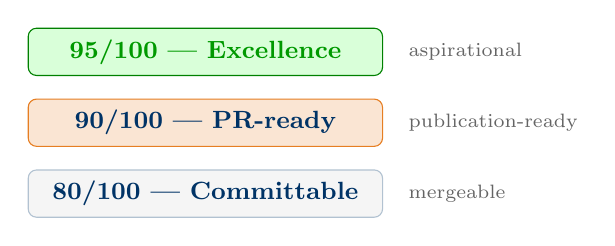
\begin{tikzpicture}[
    gate/.style={rounded corners=3pt, minimum width=4.5cm, minimum height=0.6cm,
      inner sep=4pt, font=\small\bfseries, align=center},
  ]
    \node[gate, fill=green!15, draw=green!50!black] (g3) at (0, 0) {\color{sage}95/100 --- Excellence};
    \node[gate, fill=gold!20, draw=gold] (g2) at (0, -0.9) {\color{navy}90/100 --- PR-ready};
    \node[gate, fill=lightice, draw=navy!30] (g1) at (0, -1.8) {\color{navy}80/100 --- Committable};
    \node[font=\scriptsize, text=slate, right=0.2cm of g3] {aspirational};
    \node[font=\scriptsize, text=slate, right=0.2cm of g2] {publication-ready};
    \node[font=\scriptsize, text=slate, right=0.2cm of g1] {mergeable};
  \end{tikzpicture}

  \vspace{0.1cm}
  {\small Every file scored 0--100. Nothing ships below its tier threshold.}
\end{column}
\begin{column}{0.50\textwidth}
  {\small\bfseries\color{navy} Adversarial QA loop:}
  \vspace{0.05cm}
  
\begin{tikzpicture}[
    box/.style={fill=navy, text=white, rounded corners=3pt,
      minimum width=2.5cm, minimum height=0.6cm, inner sep=4pt,
      font=\small\bfseries, align=center},
    arrow/.style={-{Stealth[length=4pt]}, gold, thick},
  ]
    \node[box] (critic) at (0, 0) {Critic};
    \node[box] (fixer) at (3.5, 0) {Fixer};
    \node[font=\scriptsize, text=slate, below=0.05cm of critic] {identifies flaws};
    \node[font=\scriptsize, text=slate, below=0.05cm of fixer] {implements fixes};
    \draw[arrow] (critic.east) -- (fixer.west);
    \draw[arrow, bend left=40] (fixer.north) to node[above, font=\scriptsize, text=slate] {up to 5 rounds} (critic.north);
  \end{tikzpicture}

  \vspace{0.1cm}
  {\small Loop continues until the Critic returns \emphsage{APPROVED} --- each round catches issues the previous one missed.}

  \vspace{0.05cm}
  \begin{keyinsight}
    {\small The \emphgold{revise-and-resubmit} model applied to code.}
  \end{keyinsight}
\end{column}
\end{columns}
\sourceref{Sant'Anna, \textit{My Claude Code Workflow}, 2026}
\end{frame}

\end{document}
